
\documentclass[ngerman]{scrreprt}  

\bibliography{references1.bib}

\usepackage{babel}


\author{Ziad Bougrine}

\usepackage{url}
\usepackage{titling}
\usepackage{graphicx}
\graphicspath{ {./pictures/} }
\usepackage{xcolor}
\usepackage{eso-pic,lipsum}
\usepackage{biblatex}
\usepackage{lmodern}
\usepackage{algorithm}
\usepackage{algpseudocode}
\usepackage{tabularx}
\usepackage{tikz}


\begin{document}
	\begin{titlepage}
		%----------------------------------------------------------------------------------------
		%	LOGO SECTION
		%----------------------------------------------------------------------------------------
		\begin{tikzpicture}[remember picture , overlay]
			\node [xshift=1cm, yshift=-5cm](a) at (current page.north west){
				
\includegraphics{fh_logo_links}};
		\end{tikzpicture}
		
		\newcommand{\HRule}{\rule{\linewidth}{0.5mm}} 
		
		\center 
		
		%----------------------------------------------------------------------------------------
		%	HEADING SECTIONS
		%----------------------------------------------------------------------------------------
		
		\textsc{\LARGE University of Applied Sciences}\\[1.5cm] 
		\textsc{\Large Seminararbeit}\\[0.5cm] 
		\textsc{FACHBEREICH09} \\
		\textsc{Angewandte Mathematik und Informatik}\\
		\vspace{4cm}
		
		%----------------------------------------------------------------------------------------
		%	TITLE SECTION
		%----------------------------------------------------------------------------------------
		
		\HRule \\[0.4cm]
		{ \huge \bfseries Blockchain- Technologie : \texttt{Analyse von Proof of Work (Bitcoin)}}\\[0.4cm] % Title of your document
		\HRule \\[1.5cm]
		
		%----------------------------------------------------------------------------------------
		%	AUTHOR SECTION
		%----------------------------------------------------------------------------------------
		
		\begin{minipage}{0.4\textwidth}
			\begin{flushleft} \large
				\emph{Author:}\\
				Ziad \textsc{Bougrine} \textit{(3560356)} \\
			\end{flushleft}
		\end{minipage}
		~
		\begin{minipage}{0.4\textwidth}
			\begin{flushright} \large
				\emph{Lecturer:} \\
				prof. dr. Volker \textsc{Sander} \\
				prof. dr. Walk \textsc{Lukas} \\
			\end{flushright}
		\end{minipage}\\[2cm]
		
		{\large \today}\\[2cm]
		
		\vfill 
		
	\end{titlepage}
	
	\newpage
	Diese Arbeit ist von mir selbständig angefertigt und verfasst. Es sind keine anderen als die angegebenen Quellen und Hilfsmittel benutzt worden. \\ \\
	Ziad Bougrine ........................................... \\
	\vspace{16cm}
	
	\begin{normalsize}
		Diese Arbeit wurde betreut von:
	\end{normalsize}
	\begin{enumerate}
		\item Prüfer : \textbf{Volker, Sander}
		\item Prüfer : \textbf{Walk, Lukas}
	\end{enumerate}	



  \begin{abstract}
  	\begin{center}
  		 \begin{LARGE}
  		\textbf{Zusammenfassung auf Deutsch }
  		\end{LARGE}
  	\end{center} 
    In diesem Bericht wurde eine umfassende Analyse der Technologie der Blockchain-Netzwerke und der Kryptowährungen auf der Basis von Proof-Of-Work durchgeführt. Die Funktionsweise von Kryptowährungen wurde detailliert untersucht und die Investitionsmöglichkeiten in diese Währungen wurden erläutert. Zudem wurden die Vor- und Nachteile von Proof-Of-Work und anderen Konsensmechanismen aufgezeigt und die Zukunftsaussichten für diese Technologien wurden diskutiert. Der Bericht bietet somit eine wertvolle Ressource für diejenigen, die sich für die Blockchain-Technologie und das Investieren in Kryptowährungen interessieren.
  \end{abstract}

	\begin{abstract}
   	\begin{LARGE}
   	\begin{center}
   		\textbf{Abstract in Englisch}
   	\end{center}
	\end{LARGE}
   	This report presents a comprehensive analysis of the technology of blockchain networks and cryptocurrency based on Proof-Of-Work. The functioning of cryptocurrency was thoroughly studied, and the investment opportunities in these currencies were explained. The pros and cons of Proof-Of-Work and other consensus mechanisms were also highlighted, and the future prospects for these technologies were discussed. This report therefore provides a valuable resource for those interested in blockchain technology and investing in cryptocurrency.

   \end{abstract}

  \tableofcontents


\chapter{Einleitung}
Blockchain ist seit den späten 2000er Jahren eine der wichtigsten Technologien im Bereich digitaler Transaktionen. Im Jahr 2008 veröffentlichte eine Person oder Gruppe von Personen unter dem Namen Satoshi Nakamoto ein Whitepaper mit dem Titel "Bitcoin: A Peer-to-Peer Electronic Cash System". Vier Monate später, am 3. Januar 2009, wurde der Genesis-Block erstellt, der den Beginn und Tag 0 des Bitcoin- und Blockchain-Netzwerks markierte. Die Blockchain wurde entwickelt, um als öffentliches Hauptbuch für Bitcoin-Transaktionen zu dienen und basiert auf der "Proof-of-Work"-Methode, um die Schaffung und den Handel von Bitcoin und anderen Kryptowährungen während der Finanzkrise 2007/08 zu unterstützen. Heutzutage gibt es viele Kryptowährungen wie Litecoin (2011), Ethereum (2015) und Dogecoin (2013).\\ \\
Die Implementierung der Blockchain in Bitcoin machte es zur ersten digitalen Währung, die das Problem der doppelten Ausgaben ohne die Notwendigkeit einer vertrauenswürdigen zentralen Behörde löst. Einer der Hauptvorteile von Blockchain ist, dass jeder erstellte Block, der einen Datensatz enthält, unveränderlich ist und seine Authentizität von der gesamten Gemeinschaft autorisierter Benutzer und nicht von einer einzigen zentralen Behörde überprüft werden kann. Das System ist daher darauf ausgelegt, die Transparenz und Rechenschaftspflicht von digitalisierten Transaktionen zu verbessern.\\ \\
Ein Beispiel: Stellen Sie sich ein Transaktionsbanksystem vor, das von einem Server oder Systemadministrator verwaltet wird. Dies könnte die Wartung des Systems, das Verwalten, Löschen und Hinzufügen von Benutzer- oder Transaktionsinformationen zur Datenbank umfassen. Es könnte auch bedeuten, dass der Administrator behauptet, dass Sie ihm 10.000 € schulden, was gefährlich ist.
Das ist der Grund, warum die Blockchain-Technologie erfunden wurde. Indem es immer für alle sichtbar im Hauptbuch aufgezeichnet wird, wenn Geld von einem Konto auf ein anderes überwiesen wird, kann jeder Benutzer die Transaktion überprüfen und sicherstellen, dass sie korrekt ist. \cite{Blockchain} \cite{blockchain_wikipedia}\\ \\


\chapter{Einführung in die Blockchain}

%##############################
%#           Section 1        #
%##############################
\section{Blockchain Definition}
Die \textbf{Blockchain} ist eine ständig wachsende Liste von Datensätzen, die in einzelnen Blöcken organisiert sind. Sie dient als öffentliches Hauptbuch, in dem Personen Datensätze einsehen und erstellen können. Jeder Block besteht aus Daten, einem Hash, dem Hash des vorherigen Blocks und einem Zeitstempel. Das Wesentliche an der Blockchain ist, dass wir spätere Transaktionen auf früheren Transaktionen aufbauen und deren Richtigkeit bestätigen können, indem wir die Kenntnis der früheren Transaktionen nachweisen. Auf diese Weise wird es unmöglich gemacht, die Existenz oder den Inhalt früherer und späterer Transaktionen zu manipulieren. Andere Teilnehmer der dezentralen Buchhaltung erkennen eine Manipulation der Blockchain an der Inkonsistenz der Blöcke. \cite{businessinsider}\\ 
\\
\\
\\
Die \textbf{Blockchain} ist ein verteiltes Hauptbuch, das sich selbst reguliert, das heißt, dass es keine Person gibt, die Kontrolle oder Veränderungen vornehmen kann. Stattdessen tragen Tausende von Benutzern, die am Blockchain-Netzwerk teilnehmen, dazu bei, es funktionsfähig zu halten. Wenn eine Person versucht, das System zu betrügen, wird sie schnell als Betrugserkennung markiert, da das gesamte Netzwerk sie überprüft. \cite{iotforall_2022}

\begin{figure}[h!]
	\centering
	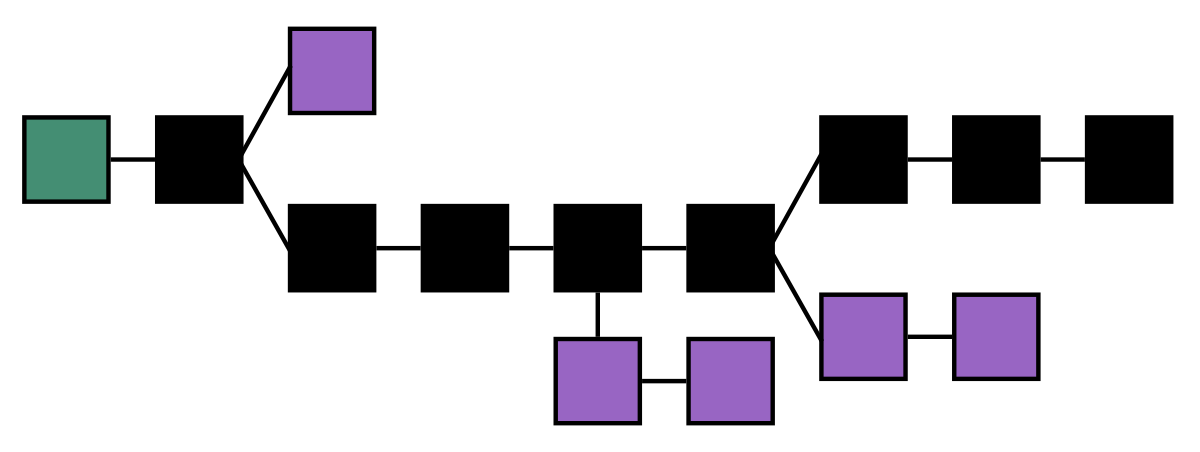
\includegraphics[width=\linewidth]{1.png}
	\caption{Ein Beispiel für eine Blockchain-Kette}
	\small URL : \url{https://de.wikipedia.org/wiki/Blockchain}
\end{figure} 


\section{Konstruktion des Blocks}
Ein Block speichert Informationen über Transaktionen, Zeitstempel, vorherigen Hash, Block-Hash.
\begin{itemize}
\item \textbf{Magische Zahl :} Nummer, die diesen Block als Teil des Netzwerks einer bestimmten Kryptowährung identifiziert.
\item \textbf{Transaktionen :} die Hauptinformationen und auch den größten Teil des Blocks
\item \textbf{Transaktionszähler :} die Anzahl der im Block gespeicherten Transaktionen
\item \textbf{Block Größe :} die maximale Größe der Informationen, die der Block enthält
\end{itemize} 
Ein Block enthält viele Informationen, belegt jedoch nicht viel Speicherplatz. Nehmen wir diese Elemente als Beispiel:
Was ist die Hauptinformationen, die ein Block (Transaktionen) enthält?
\begin{itemize}
\item \textbf{Version:} Sie ist benutzbar, um einen neuen Block zu erstellen und um eine neue Version von Software zu identifizieren. Es ist auf 4 Bytes (4 x 8 „bits“) codiert.
\item \textbf{Vorheriger Block-Hash:} Enthält einen Hash des Headers des vorherigen Blocks (md5, sha256 ...). Es ist auf 32 Bytes (32 x 8 = 256 „bits“) codiert.
\item \textbf{Hash Merkle root:} Hash of transactions in the Merkle tree of the current block. Es ist auf 32 Bytes (32 x 8 = 256 „bits“) codiert.
\item \textbf{Time:} Erstellungszeit des Blocks. Es ist auf 32 Bytes (32 x 8 „bits“) codiert.
\item \textbf{Bits:} Es ist ein Wert, der die Schwierigkeitsbewertung des Ziel-Hashes und die Schwierigkeit beim Lösen der „Nonce“ angibt. Es ist auf 32 Bytes (32 x 8 „bits“) codiert.
\item \textbf{Nonce:} Es ist die magische Zahl, die der Miner lösen muss, um einen Block im Blockchain-Netzwerk zu verifizieren und zu schließen.\\ \\
\end{itemize}

\color{green}
\Large{\textbf{Information :}} 
\color{black}
\normalsize
Die Miner setzen ihre Rechenleistung ein, um mithilfe von Zufallszahlen (Bruteforce) die Nonce im Hash zu erraten. Sobald die Nonce erfolgreich bestimmt wurde, wird der Hash verifiziert und der Block geschlossen. Anschließend wird ein neuer Block mit einem Header erstellt und der Prozess wiederholt sich. Die Nonce ist von Interesse für Miner, da sie einen wichtigen Bestandteil des Mining-Prozesses darstellt, bei dem versucht wird, den Hash zu lösen. \\ \\ \\

\large
\newpage
\underline{\textbf{Was sind Merkle-Bäume?}} \\ \\
\normalsize
Es handelt sich um eine Datenstruktur in Form eines Binärbaums, die in Bitcoin und Kryptowährung weit verbreitet ist und zur effizienten und sicheren Kodierung von Daten verwendet wird.




\section{Blockchaining-Mechanismus}
\textbf{Die Funktionsweise der Blockchain} ähnelt der einer verketteten Liste, da sie aus einer Reihe von Blöcken besteht, die jeweils durch einen Hash des aktuellen Blocks und einen Hash des vorherigen Blocks verbunden sind. Dieser Mechanismus ermöglicht es, über die Kette zu iterieren, ähnlich wie bei einer verketteten Liste, in der jeder Knoten einen Zeiger auf den vorherigen Knoten enthält. \cite{fool}

\begin{figure}[h!]
	\centering
	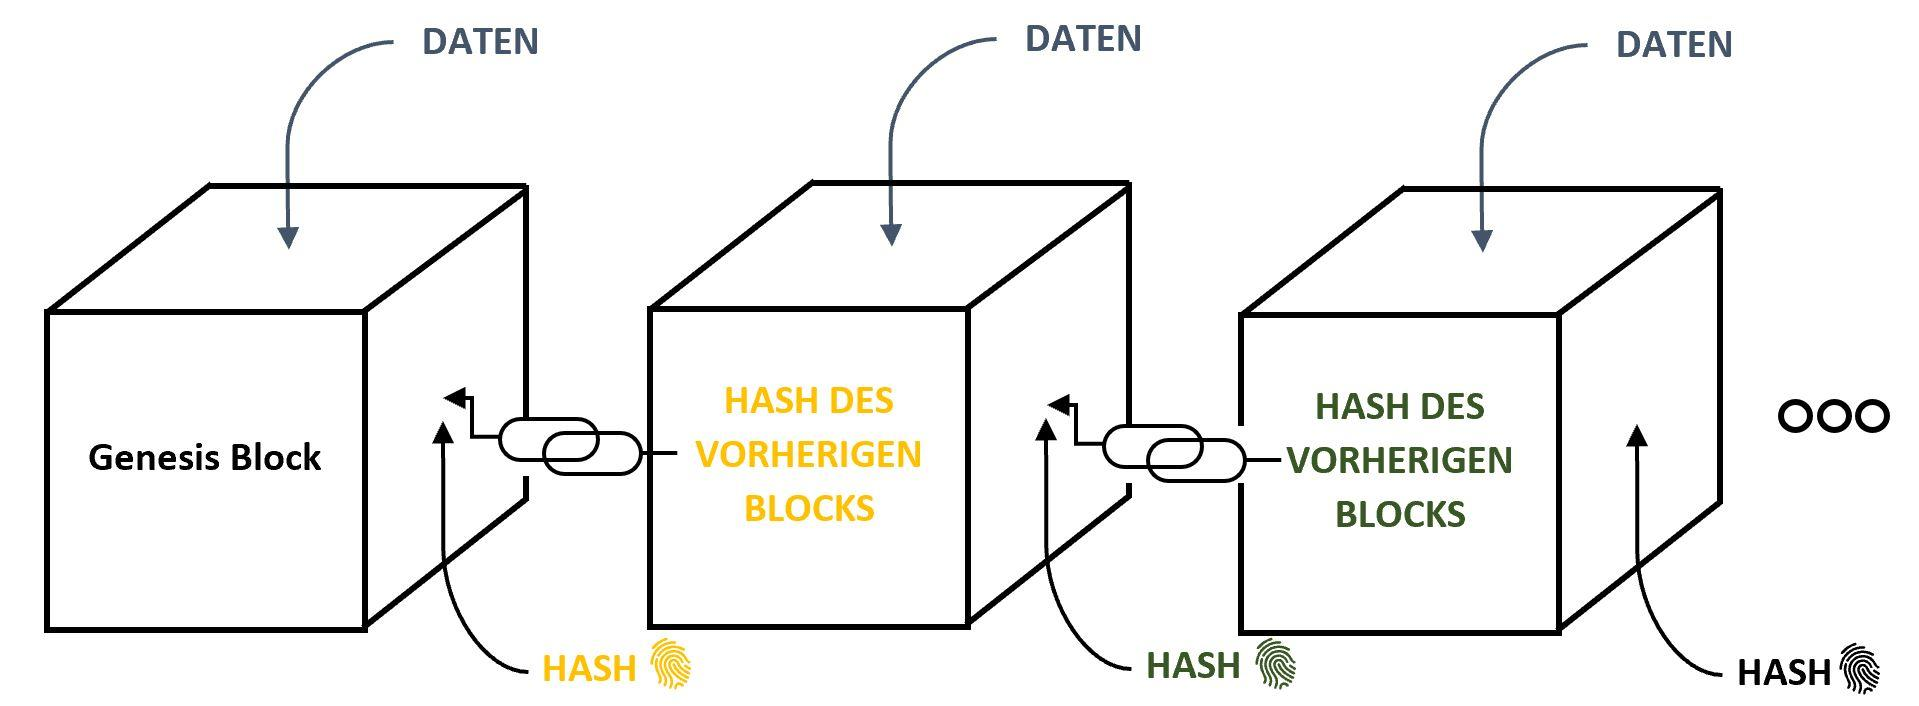
\includegraphics[width=\linewidth]{2.jpg}
	\caption{Der erste Block der Kette wird als Genius-Block bezeichnet.}
	\small URL : \url{https://muenchen.digital/wp-content/uploads/Blockchain-1.jpg}
\end{figure} 
In solchen Fällen sollte man immer bedenken, welche Handlungen von verdächtigen Personen ausgehen könnten, beispielsweise das Modifizieren oder Manipulieren der Daten im Block (i). Dies führt zu einer Änderung des tatsächlichen Blocks i und macht den vorherigen Hash im Block (i+1) ungültig. Dies bedeutet, dass das Ändern eines Blocks alle darauf folgenden Blöcke in der Blockchain ungültig macht, was die Integrität der Kette beweist.\\ \\
\color{red}
\Large{\textbf{Achtung :}}
\color{black}
\textbf{Ist dieser Mechanismus gesichert?}\\
\normalsize
 	
Der Einsatz von Hashes allein reicht nicht aus, um Manipulationen zu verhindern. Da Computer heutzutage sehr schnell sind und Tausende von Hashes berechnen können, besteht technisch gesehen die Möglichkeit, einen Block zu manipulieren und alle nachfolgenden Hashes der nachfolgenden Blöcke erneut zu berechnen, um das Blockchain-Netzwerk wieder gültig zu machen. Aus diesem Grund verwendet die Blockchain den sogenannten "Proof of Work (POW)", um dieses Problem zu vermeiden.	



\chapter[Theoretische Seite der Proof-Of-Work-Methode]{Einführung in die „Proof-Of-Work“-Methode}	

\section{Was ist Proof-Of-Work ?}
Proof-Of-Work (POW) wurde entwickelt, um zu verhindern, dass Nutzer Blocks in der Blockchain leicht manipulieren. Es verlangt von Minern, eine signifikante Menge an Mühe aufzuwenden, um einen Block zu erstellen. Diese Methode basiert auf verschiedenen Grundprinzipien in der Kryptowährung \cite{proof_of_work_wikipedia}, wie folgt:

\begin{itemize}
	\item{Der Proof-of-Work-Mechanismus sorgt dafür, dass das Hinzufügen von Blöcken zur Blockchain-Kette mit einer gewissen Schwierigkeit verbunden ist, indem es Miner dazu zwingt, einen gültigen Hash zu finden. Diese Methode wurde so konzipiert, dass etwa alle zehn Minuten ein neuer Block mit einer festgelegten Menge an BTC in die Kette aufgenommen wird. Dies gewährleistet das algorithmische Wachstum der Geldmenge. \cite{btc-echo-proof-of-work}}
	\item{Die Verwendung von Proof-of-Work ermöglicht es den Nodes, die Integrität der Blockchain zu überprüfen, indem sie diejenige wählen, die den größten Aufwand in Form von Rechenleistung darstellt. Auf diese Weise ist es einfach zu erkennen, welche Blockchain die authentische ist.}
	\item{Die Verwendung von Proof of Work dient dazu, das Blockchain-Netzwerk vor Angreifern zu schützen, da diese eine größere Energiemenge in das Netzwerk einspeisen müssten als alle anderen verfügbaren Miner insgesamt über einen längeren Zeitraum. Dies ist beim Bitcoin aufgrund der enormen Rechenleistung, die benötigt wird, um einen gültigen Block zu erstellen, praktisch unmöglich.}
	\item{Proof of Work ist eine bewährte Methode zur Sicherung von Blockchains und zur Neuverteilung von digitalen Währungen. Im Gegensatz zu Fiatgeld, das von Zentralbanken gedruckt werden kann, erfordert die Erschaffung von Coins in einem Proof-of-Work-System einen tatsächlichen Einsatz von Ressourcen. Dadurch wird ein fairer Mechanismus für die Verteilung von Coins gewährleistet. \cite{btc-echo-proof-of-work}}
\end{itemize}

\section{Wie funktioniert Proof of Work bei einer Blockchain ?}
Der Proof-of-Work-Mechanismus erfordert, dass Miner mithilfe von Bruteforce-Methoden versuchen, eine Nonce zu finden, die bestimmte Eigenschaften aufweist, wodurch Milliarden von Berechnungen durchgeführt werden. Sobald ein solches Ergebnis erzielt wurde, wird den Minern eine Belohnung in Form einer Blocksubvention gewährt. Dieser Prozess wird als Mining bezeichnet.\\ \\ \\ \\
\textbf{Diese beschreiben den Prozess einer Transaktion im Blockchain-Netzwerk. \\ }
\begin{itemize}
	\item{Die Blockchain generiert einen Block, der alle Transaktionen enthält, die in einem bestimmten Zeitraum stattgefunden haben.}
	\item{Der Verifizierer wird die Integrität der Transaktionen überprüfen, um sicherzustellen, dass sie legitim sind. \cite{btc-echo-proof-of-work}}
	\item{Die Miner im Netzwerk überprüfen dann die Legitimität dieser Transaktionen und führen anschließend eine Suche durch, indem sie die Nonce erraten. Der erfolgreiche Miner, der als erstes die Lösung findet, wird mit einer Belohnung und den Transaktionsgebühren belohnt. Dieser Prozess wird als "Mining" bezeichnet. Das Blockchain-Netzwerk wird dann um den Block mit den bestätigten Transaktionen erweitert und wird als Teil der Kette von Blöcken gespeichert.\cite{btc-echo-proof-of-work}}
	\item{Die Transaktionsbestätigung im Blockchain-Netzwerk wird wiederholt \\}
	
\end{itemize}
\textbf{Dies ist ein sequentielles Diagramm, das erklärt, wie es funktioniert \\}
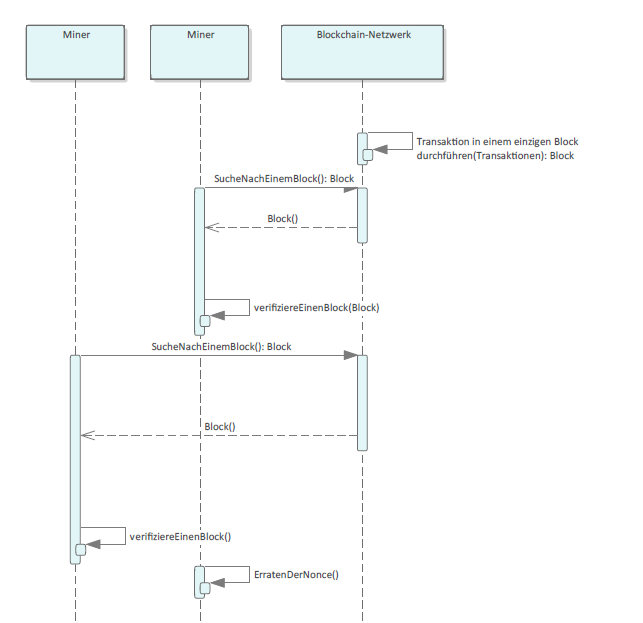
\includegraphics[width=\linewidth]{ProofOfWork1.png} \\ \\
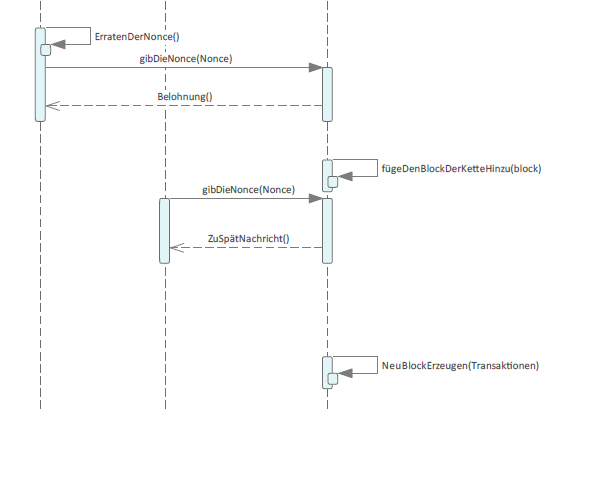
\includegraphics[width=\linewidth]{ProofOfWork2.png}
\section{Wie genau funktionieren die Proof-of-Work-Berechnungen?}
\begin{itemize}
	\item {Die Miner im Blockchain-Netzwerk nutzen Hash-Funktionen, die in ihrer Funktionsweise unumkehrbar sind. Sie können eine beliebig lange Zeichenfolge in eine eindeutige Zeichenfolge festgelegter Länge umwandeln. Die Schwierigkeit besteht darin, ein Ergebnis zu erzielen, das bestimmte Eigenschaften aufweist, die sich aus der Verwendung der Hash-Funktion ergeben. Ein bekanntes Beispiel hierfür ist der Einsatz der SHA-256-Hash-Funktion im Bereich des Minings bei Bitcoin. \cite{btc-echo-proof-of-work}}
	\item{Die Hash-Funktion ist eine eindeutige, nicht invertierbare mathematische Funktion, die aus einer beliebigen Eingabestring eine feste Länge erzeugt. Sie wird häufig in der Kryptographie und im Blockchain-Bereich verwendet. Im Fall von Kryptowährungen wie Bitcoin wird sie beim Mining verwendet, wobei Miner versuchen, einen Wert mit bestimmten Eigenschaften zu finden, indem sie der Hash-Funktion Zeichenfolgen übergeben. Da die Rückgängigmachung der Hash-Funktion nicht möglich ist, kann der Miner den erhaltenen Wert nicht einfach umkehren und die Eingabe der Hash-Funktion erhalten.} \cite{fool}, \cite{btc-echo-proof-of-work}
	\item{Aus diesem Grund gibt es das Konzept \textbf{"Mining"}, Mining ist ein Prozess, bei dem Miner versuchen, die Nonce und die Reihenfolge der Parameter zu erraten, die von einer Hash-Funktion als Eingabe akzeptiert werden, um ein Ergebnis zu liefern. Da es unmöglich ist, die Hash-Funktion umzukehren, um die ursprüngliche Eingabe zu erhalten, müssen Miner eine Vielzahl von Operationen durchführen, um den Wert der Eingabe für die Hash-Funktion zu ermitteln. Dies geschieht durch das Konzept des Minings, bei dem Miner versuchen, die Nonce und die Reihenfolge jedes Parameters, die von der Hash-Funktion als Eingabe akzeptiert werden, zu erraten.}
	\item{Wenn der Block abgebaut wird, überprüfen alle Teilnehmer des Blockchain-Netzwerks die präsentierte Lösung, um zu bestätigen, dass die Gültigkeit der Blockchain aufrechterhalten wird.} \cite{btc-echo-proof-of-work} 
\end{itemize}


\section{Was hat es mit der Schwierigkeit auf sich ?}
\begin{itemize}
\item{Die Schwierigkeit besteht darin, die gewünschte Hash-Ausgabe zu finden. Zum Beispiel Bitcoin, es wird eine Frage gestellt: Wie viele Nullen soll die Ausgabe am Anfang des Strings haben. Je mehr Nullen gefordert sind, desto schwieriger wird es schließlich, den Output zu finden. \cite{btc-echo-proof-of-work}}
\item{Die Schwierigkeit ist bei Bitcoin immer so gewählt, dass im Schnitt alle zehn Minuten ein neuer Block gefunden werden soll. Dieser Benchmark wird alle zwei Wochen überprüft. Stellt sich heraus, dass in zwei Wochen der Richtwert von 2.016 Blöcken überschritten wurde, also mehr Blöcke als gewünscht gefunden wurden, ist die Schwierigkeit zu gering und wird nach oben korrigiert – und umgekehrt. \cite{btc-echo-proof-of-work}}
\end{itemize}
\section{Sicherheit des Proof-Of-Work}

\begin{itemize}
	\item Der Proof-of-Work ist eine Technik, die in vielen Kryptowährungen eingesetzt wird, um Transaktionen zu verifizieren und neue Blöcke in die Blockchain einzufügen. Miner müssen dabei bestimmte Berechnungen durchführen, um einen neuen Block zu "abbauen" und somit eine Belohnung zu erhalten.
	
	\item Der Proof-of-Work bietet eine gewisse Sicherheit, da es für Angreifer schwierig ist, die Blockchain zu verändern, ohne die erforderliche Rechenleistung zu erbringen. Allerdings gibt es auch Nachteile, wie hohe Energiekosten und langsamere Transaktionsgeschwindigkeiten im Vergleich zu anderen Konsensmechanismen.
\end{itemize}
\section{Vor- und Nachteile von Proof-Of-Work}
\textbf{Um die Vor- und Nachteile dieser Methode genau zu erklären, wurde diese Tabelle erstellt: \cite{fool} } \\ \\
\begin{tabular}{|c|c|}
	\hline
	\textbf{Vorteile} & \textbf{Nachteile} \\ \hline
	Sicherheit & Hohe Energiekosten \\ \hline
	Gute Anreizstruktur & Langsame Transaktionsgeschwindigkeiten \\ \hline
	Breite Akzeptanz & Mögliche Zentralisierung von Mining-Pools \\ \hline
	Verteilte Konsensfindung & Hardware-Anforderungen \\ \hline
\end{tabular}\\ \\
\textbf{\underline{Eklärung :}}
\begin{itemize}
	\item \textbf{Sicherheit :}
	\begin{itemize}
		\item Um ein hohes Sicherheitsniveau in einem auf Proof-of-Work basierenden Blockchain-Netzwerk zu gewährleisten, müsste eine spekulative Person die Kontrolle über die Mehrheit der Mining-Kapazität erlangen. Dies würde bedeuten, dass sie mindestens 50\% des Netzwerks besitzen müsste, was aufgrund der verteilten Natur von Proof-of-Work-Systemen als unmöglich gilt. Eine solche Person benötigte auch eine beträchtliche Menge an Hardware und Energie, um in der Lage zu sein, die benötigte Rechenleistung zu erbringen.
		
		\item Ein "51\%-Angriff" stellt eine Sicherheitsmaßnahme dar, die verhindern soll, dass eine spekulative Person die Kontrolle über ein auf Proof-of-Work basierendes Blockchain-Netzwerk übernimmt. Um ein solcher Angriff zu verhindern, müsste die Person mindestens 50\% der Mining-Kapazität besitzen, was aufgrund der dezentralisierten Natur von Proof-of-Work-Systemen als unmöglich gilt.
		
		\item Es gibt jedoch auch andere Faktoren, die die Sicherheit von Proof-of-Work-Systemen beeinflussen. Dazu gehören die Größe und Zentralisierung von Mining-Pools, die Sicherheit von Hardware und die Implementierung des Konsensmechanismus. Um das Sicherheitsniveau eines Proof-of-Work-Systems vollständig zu verstehen, ist es wichtig, diese Faktoren zu berücksichtigen.
	\end{itemize}
	\item \textbf{Gute Anreizstruktur :}
	\begin{itemize}
		\item Eine gut ausgelegte Anreizstruktur ist ein wesentlicher Faktor für den Erfolg eines Proof-of-Work-Systems. Miner erhalten eine finanzielle Belohnung für das Lösen von Rechenaufgaben und die damit verbundenen Bemühungen, die als Anreiz dienen, ihre Rechenleistung bereitzustellen und somit die Integrität und Sicherheit der Blockchain zu gewährleisten.
		
		\item Eine gute Anreizstruktur kann auch dazu beitragen, das Gleichgewicht des Systems aufrechtzuerhalten und die Beteiligung von Miner zu fördern. Wenn die Belohnungen für das Mining zu gering sind, könnten Miner weniger motiviert sein, ihre Rechenleistung zur Verfügung zu stellen, was zu einer Beeinträchtigung der Sicherheit führen könnte. Auf der anderen Seite könnten zu hohe Belohnungen dazu führen, dass das System unausgeglichen wird und es zu einer Zentralisierung von Mining-Pools kommt.
		
		\item Es ist wichtig, dass die Anreizstruktur von Proof-of-Work-Systemen sorgfältig abgestimmt ist, um eine ausgeglichene Beteiligung von Miner und ein hohes Sicherheitsniveau zu gewährleisten.
	\end{itemize}
	
	\item \textbf{Verteilte Konsensfindung :} Die dezentralisierte Konsensbildung ist ein wichtiger Aspekt von Blockchain-Systemen, die nicht von einer zentralen Stelle kontrolliert werden, wie dem Proof-of-Work. Bei diesem Verfahren werden Transaktionen von allen Teilnehmern des Netzwerks überprüft, anstatt von einer zentralen Institution wie einer Bank oder Regierung. \\
	
	\item \textbf{Belohnung} Viele Menschen schätzen Bitcoin aufgrund der Möglichkeit, an der Mining-Operation teilzunehmen. Dazu können sie spezielle Hardware, sogenannte "Rig Mining"-Geräte, einrichten und damit mit dem Abbau von Bitcoin beginnen. Für jeden erfolgreichen Abbauvorgang erhalten sie eine Belohnung in Form von Bitcoin. Die Möglichkeit, an der Mining-Operation teilzunehmen, macht Bitcoin für viele Menschen attraktiv und gibt ihnen die Möglichkeit, daran zu verdienen. Es ist jedoch wichtig zu beachten, dass das Mining von Bitcoin auch mit hohen Energiekosten und möglichen technischen Herausforderungen verbunden ist. \\ 
\end{itemize}
\textbf{Obwohl der Proof-of-Work ein wichtiger Konsensmechanismus in vielen Kryptowährungen ist, gibt es auch einige Nachteile, die berücksichtigt werden sollten.}
\begin{itemize}
	\item Transaktionen sind so langsam, weil sie eine Menge von Mining-Operationen benötigen, um einen Block zu überprüfen, der Bitcoin-Transaktionen enthält, auch Blockchain Durchschnitt der Suche nach einem Block nonce ist 1 Nonce pro 10 Minuten, die es so langsam für einen großen Market ist.
	\item \textbf{Hohe Energiekosten :}
	\begin{itemize}
		\item Der Betrieb eines auf Proof-of-Work basierenden Blockchain-Netzwerks kann mit hohem Energiebedarf verbunden sein, da Miner Rechenleistung bereitstellen müssen, um neue Blöcke zu erstellen und Transaktionen zu validieren. Dies erfordert häufig die Verwendung von spezialisierten Mining-Geräten, die viel Strom verbrauchen und möglicherweise auch Kühlsysteme benötigen, um hohe Temperaturen zu vermeiden.
		
		\item Eine Möglichkeit, den Energiebedarf von Mining-Operationen zu reduzieren, besteht darin, erneuerbare Energien zu nutzen, um den benötigten Strom zu erzeugen. Dies kann zwar höhere Anfangsinvestitionen erfordern, aber es bietet auch langfristige Vorteile, da Mining-Unternehmen keinen externen Strom verbrauchen und somit keine Energiekosten haben. Erneuerbare Energien wie Solar- und Windenergie können eine umweltfreundliche Alternative zu fossilen Brennstoffen darstellen und können dazu beitragen, den CO2-Ausstoß von Mining-Operationen zu reduzieren.
		
		\item Es ist wichtig, den Energiebedarf von Mining-Operationen sorgfältig zu berücksichtigen, um sicherzustellen, dass sie nachhaltig und umweltfreundlich sind. Wenn zu viele Miner ohne Rücksicht auf den Energieverbrauch minen, könnten die Energiepreise steigen und die Umwelt belasten. Daher ist es wichtig, dass Miner ihren Energieverbrauch sorgfältig planen und, falls möglich, erneuerbare Energien nutzen.
	\end{itemize}
	
	\item \textbf{Langsame Transaktionsgeschwindigkeiten :}
	\begin{itemize}
		\item Eines der Haupthindernisse für die Schnelligkeit von Bitcoin-Transaktionen ist die Tatsache, dass sie von Minern validiert werden müssen, um in die Blockchain aufgenommen zu werden. Dies erfordert, dass Miner bestimmte Rechenaufgaben lösen, um einen neuen Block zu erstellen, der die Transaktionen enthält. Da die Schwierigkeit, einen neuen Block zu finden, von Zeit zu Zeit angepasst wird, kann es durchaus eine Weile dauern, bis ein Block gefunden wird.
		
		\item Die durchschnittliche Zeit, die benötigt wird, um einen neuen Block zu finden, beträgt derzeit etwa 10 Minuten. Dies bedeutet, dass es in der Regel etwa 10 Minuten dauern wird, bis eine Transaktion bestätigt wird und in die Blockchain aufgenommen wird. Für einige Benutzer könnte dies als langsam empfunden werden, insbesondere im Vergleich zu traditionellen Zahlungsmethoden.
		
		\item Es gibt jedoch auch Maßnahmen, die getroffen werden können, um die Schnelligkeit von Bitcoin-Transaktionen zu verbessern, wie zum Beispiel die Verwendung von Segregated Witness (SegWit) oder Lightning-Netzwerken. Diese Technologien können die Größe von Transaktionen reduzieren und somit die Geschwindigkeit erhöhen. 
				
	\end{itemize}
	\begin{figure}[h!]
		\centering
		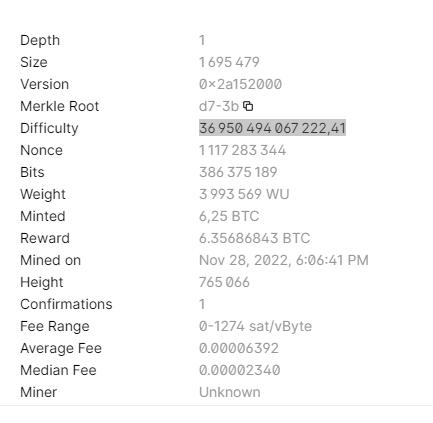
\includegraphics[width=7cm,height=7cm]{difficulty}
		\caption{Die heutige Schwierigkeit ist}
		\small URL : \url{https://www.blockchain.com/explorer/api/blockchain_api}
	\end{figure} 
	
	\item \textbf{Hardware-Anforderungen :}
	\begin{itemize}
		\item Das Abbauen von Bitcoin kann hohe Investitionskosten erfordern, da es oft notwendig ist, spezielle Mining-Hardware wie leistungsstarke Grafikkarten und entsprechende Motherboards zu beschaffen, um erfolgreich neue Blöcke zu erstellen. Die hohen Preise für diese Ausrüstung können es schwierig machen, in das Bitcoin-Mining einzusteigen, insbesondere für Einzelpersonen oder kleine Unternehmen.
		
		\item Trotzdem kann das Bitcoin-Mining dennoch lukrativ sein, insbesondere für größere Mining-Unternehmen mit mehreren Mining-Geräten und Zugang zu günstigem Strom. In diesen Fällen können die Einnahmen aus dem Mining die Investitionskosten schnell übersteigen und eine rentable Einkommensquelle darstellen.
		
		\item Es ist wichtig zu beachten, dass das Bitcoin-Mining auch ein hochvolatiles Unterfangen sein kann, da der Wert von Bitcoin und damit auch die Belohnungen für das Mining stark schwanken können. Daher ist es wichtig, sorgfältig zu planen und das Risiko sorgfältig abzuwägen, bevor man in das Bitcoin-Mining investiert.
	\end{itemize}
	
	
\end{itemize}

\chapter[Praktische Anwendung der Proof-Of-Work-Methode]{Algorithmus zur Bestimmung der Nonce in Kryptowährungen}
\begin{figure}[H]
	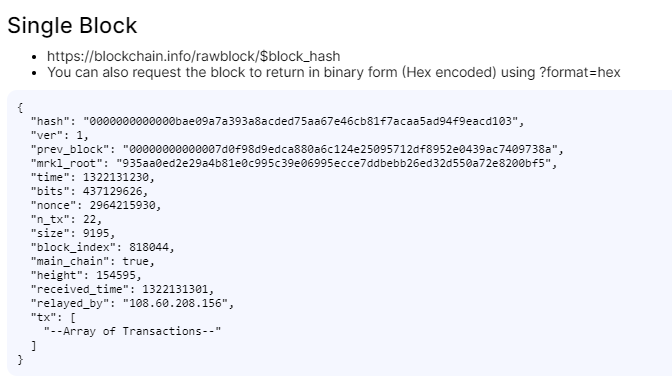
\includegraphics[width=\linewidth,height=6cm]{realblock.png}
	\caption{Es ist von Interesse, die technische Funktionsweise von Proof-of-Work zu untersuchen. Als Erstes betrachten wir eine tatsächliche Blockstruktur von der offiziellen Website.}
\end{figure}
\begin{figure}[H]
	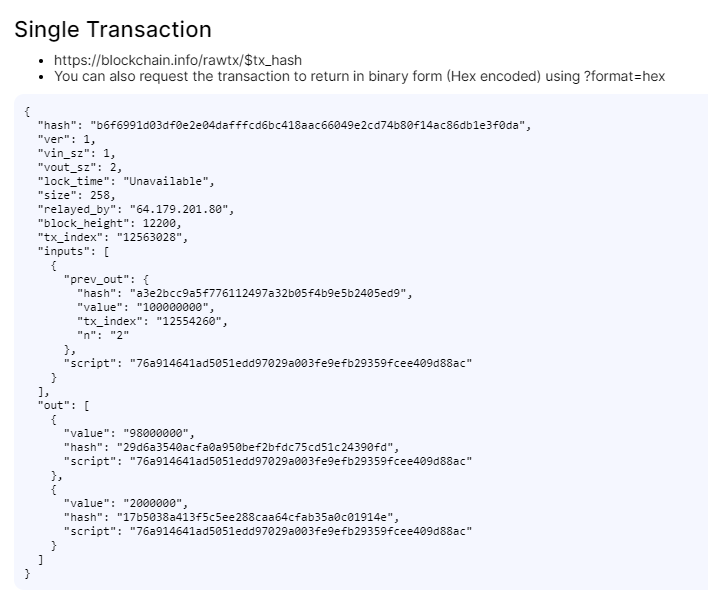
\includegraphics[width=\linewidth,height=6cm]{realtransaction.png}
	\caption{Die echten Blockchain-Block-Transaktionen.}
	
\end{figure}
\newpage
\begin{figure}[H]
	\centering
	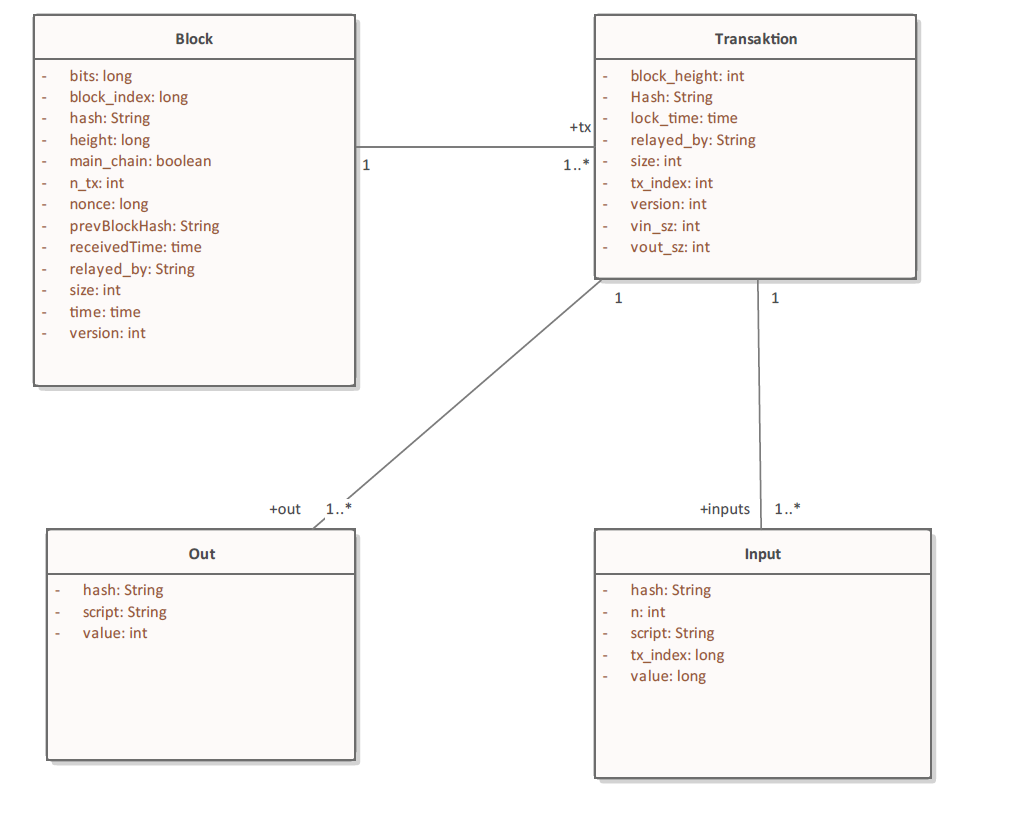
\includegraphics[width=\linewidth]{classOfStructures.png}
	\caption{Das nächste Diagramm, das als Klassendiagramm bezeichnet wird, gibt eine visuelle Darstellung aller Daten, die im realen Blockchain-Netzwerk enthalten sind. Dieses Diagramm ist hilfreich, um die Implementierung des Blockchain-Netzwerks besser zu verstehen und zu analysieren. Es zeigt die Beziehungen und Abhängigkeiten zwischen den verschiedenen Elementen des Netzwerks und hilft, die Struktur und Funktionsweise des Systems zu verdeutlichen. Die Verwendung eines Klassendiagramms ermöglicht es, die komplexen Zusammenhänge einfacher darzustellen und die Implementierung des Blockchain-Netzwerks besser zu verstehen.}
\end{figure}
\newpage
\begin{figure}[H]
	\centering
	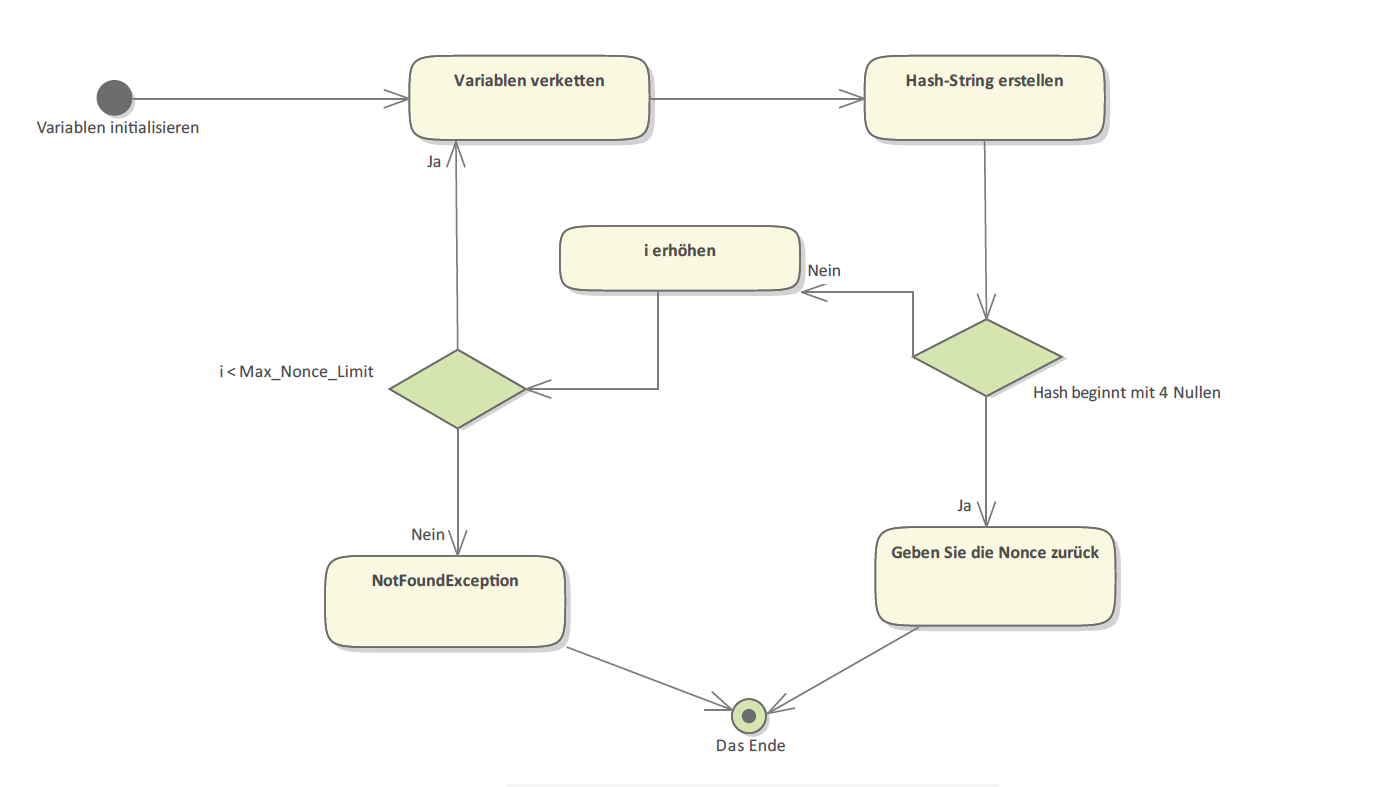
\includegraphics[width=\linewidth]{activity.png}
	\caption{Der Algorithmus zur Bestimmung der Nonce wird mit dem Aktivitätsdiagramm erklärt. Zunächst müssen wir die initialen Daten initialisieren, einschließlich des MaxNonceLimit, der Anzahl der Nullen, die der Hash haben sollte. In diesem Beispiel betrachten wir die Anforderung, dass der Hash mit 4 Nullen beginnen sollte. Es ist wichtig zu beachten, dass die Anzahl der Nullen eine wichtige Rolle bei der Bestimmung der Komplexität des Algorithmus spielt. Je höher die Anzahl der Nullen, desto länger wird es dauern, die Nonce mit begrenzter Hardware zu finden. Wir sollten auch unsere Inkrementierungsvariable für die for-Schleife initialisieren.}
\end{figure}

\textbf{Dies ist der Algorithmus \textcommabelow der für dieses Beispiel zum Schürfen von Bitcoin geschrieben wurde} \\
\begin{algorithm}
	\caption{Nonce für gültigen Hash finden}
	\label{alg:nonce_find}
	
	\begin{algorithmic}[1]
		\State nonce $\gets$ 0
		\Repeat
		\State hash $\gets$ Hash(block\_data, nonce)
		\If{hash meets difficulty level}
		\State \textbf{return} nonce
		\EndIf
		\State nonce $\gets$ nonce + 1
		\Until{hash meets difficulty level}
	\end{algorithmic}
\end{algorithm}

\chapter{Der Bitcoin-Markt und die Verwendung von Proof of Work}
\section{Kryptowährungen, auf die Proof-Of-Work basieren}

	Einige der bekanntesten Kryptowährungen, die den Konsensmechanismus Proof-Of-Work verwenden, sind Bitcoin, Bitcoin Cash, Bitcoin Sv, Litecoin und Dogecoin. \\
		
	\begin{figure}[H]
		\centering
		
\includegraphics[width=1.5cm,height=1.5cm]{bitcoincash.png}
		\caption{Bitcoin Cash}
		\small URL : \url{https://upload.wikimedia.org/wikipedia/commons/5/58/Bitcoin_Cash.png}
	\end{figure} 
	\begin{figure}[H]
		\centering
		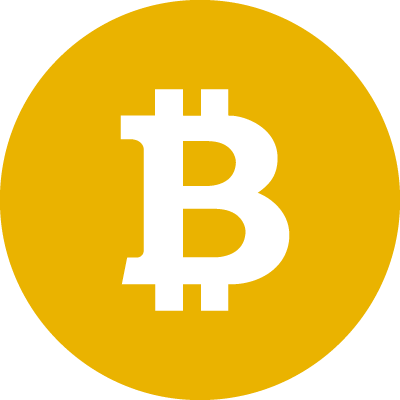
\includegraphics[width=1.5cm,height=1.5cm]{bitcoinsv.png}
		\caption{Bitcoin SV}
		\small URL : \url{https://upload.wikimedia.org/wikipedia/commons/c/c1/Bsv-icon-small.png}
	\end{figure}
	\begin{figure}[H]
		\centering
		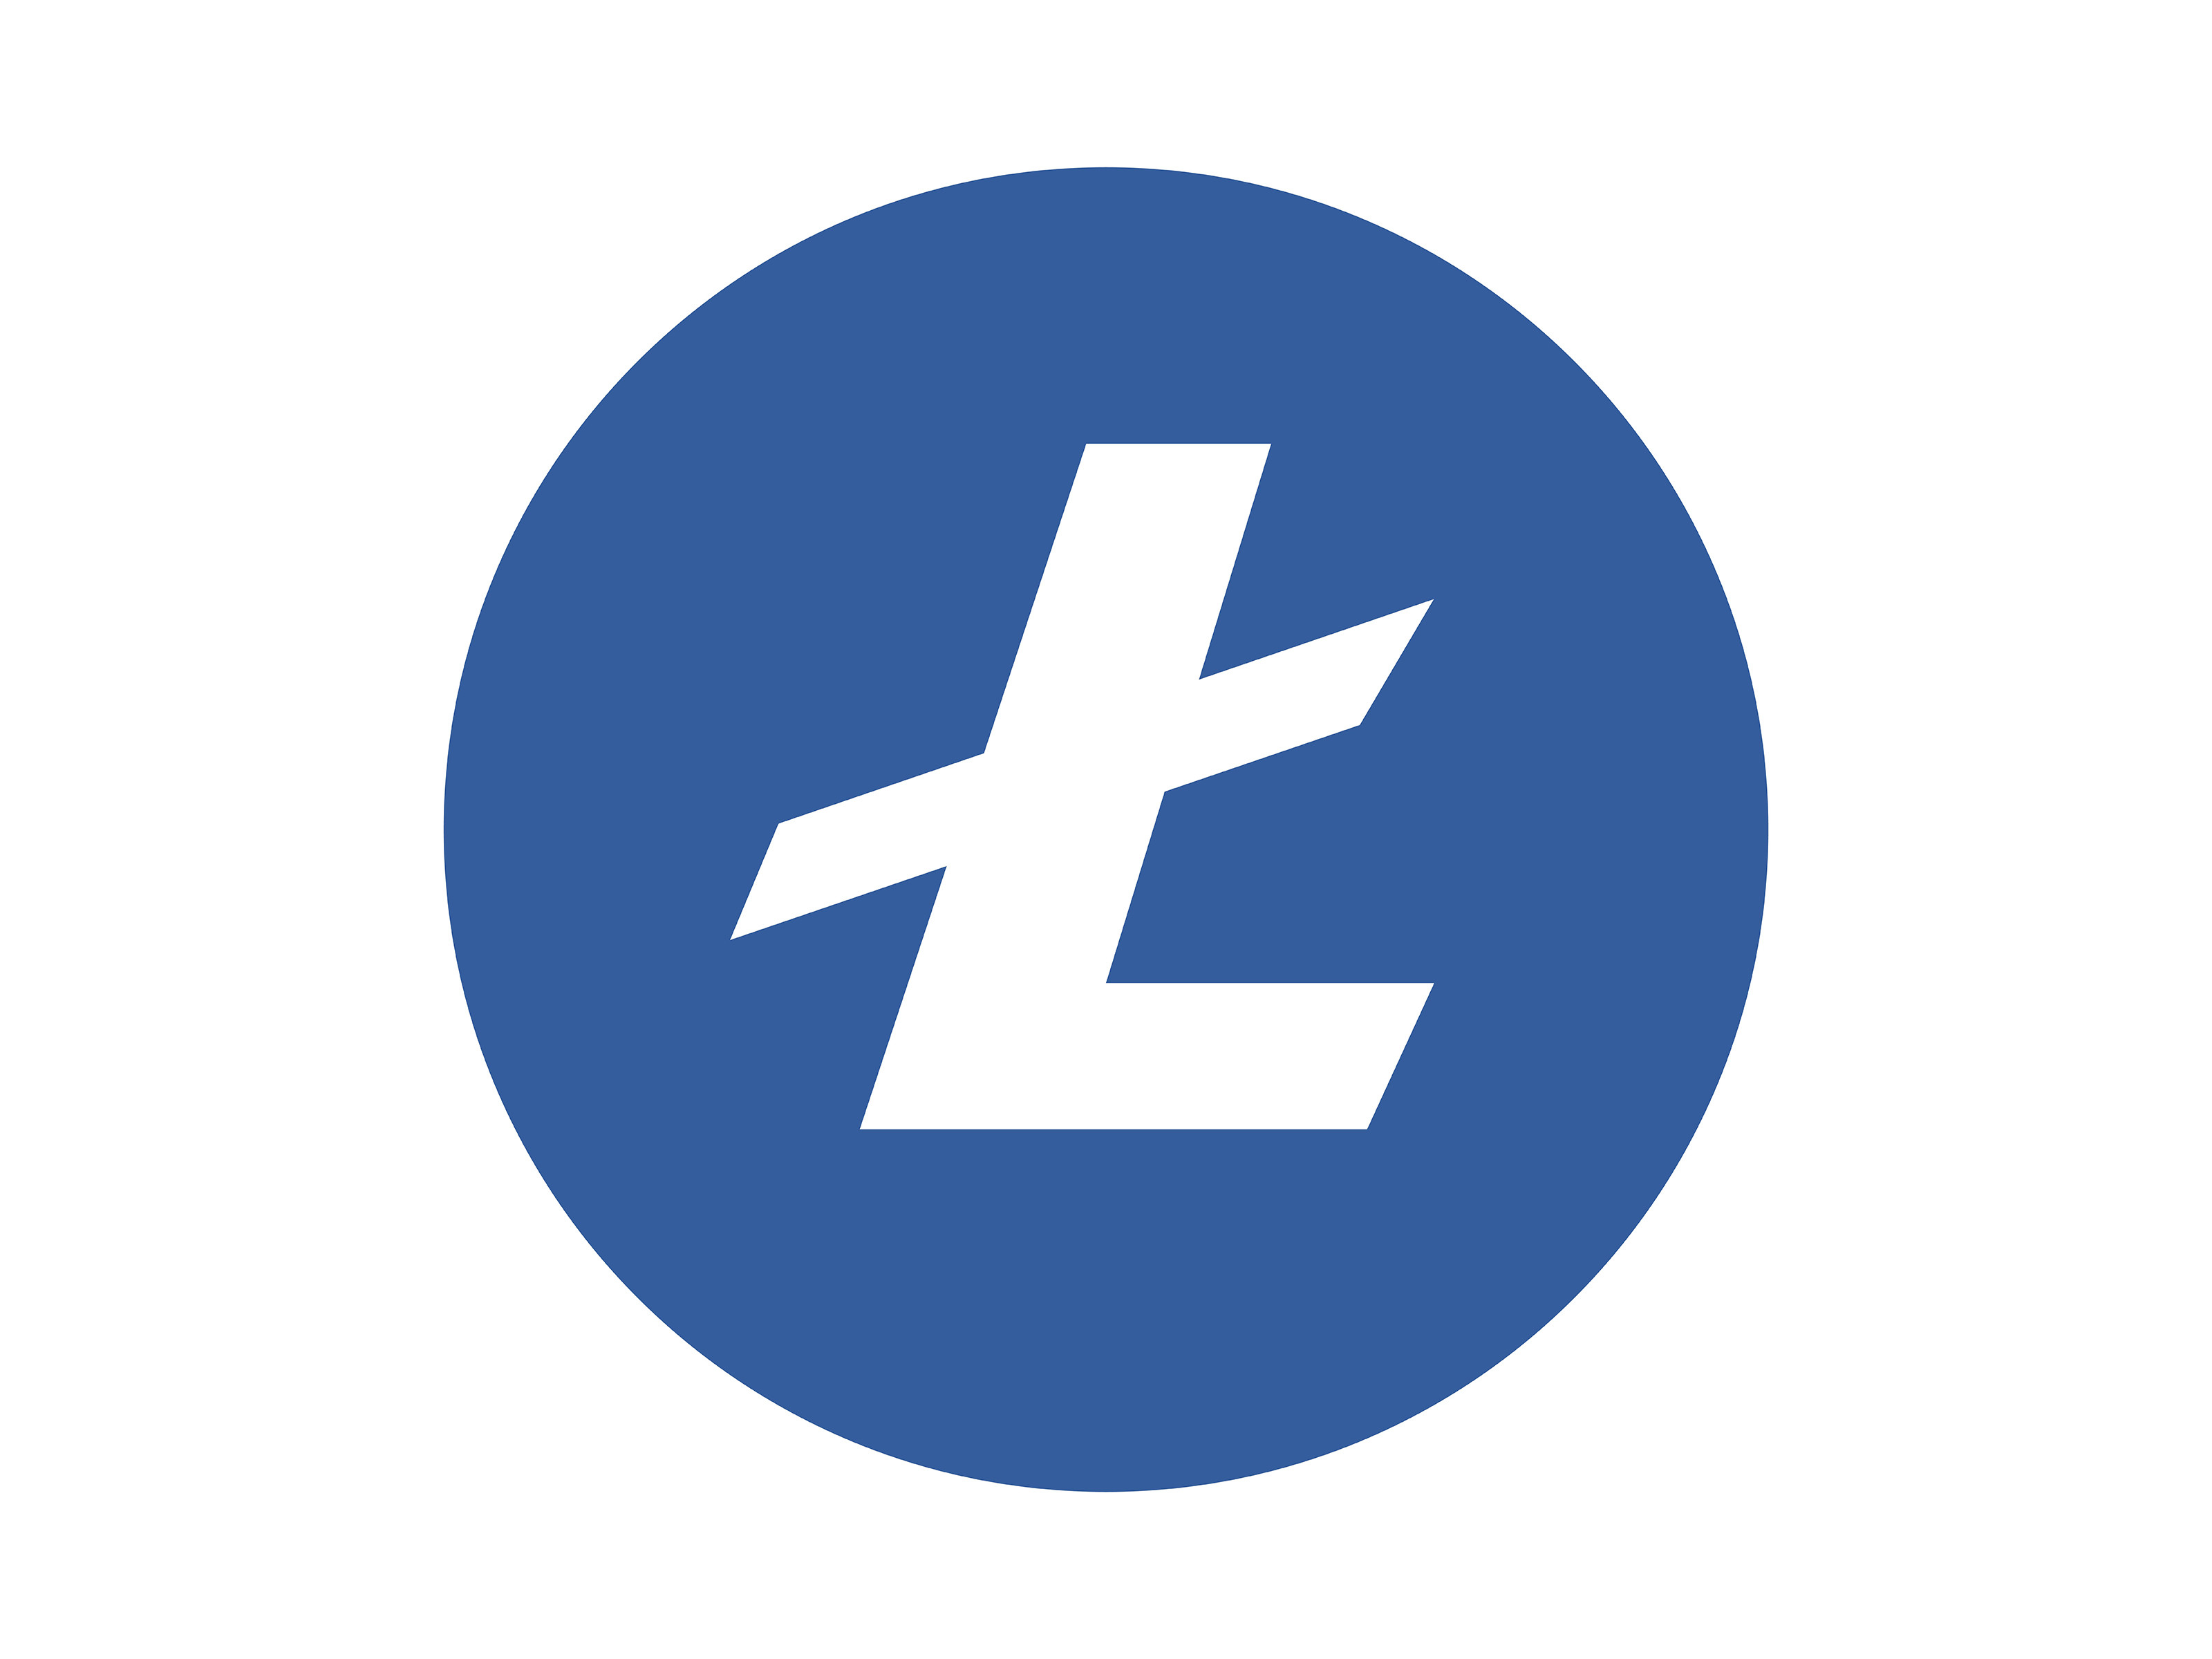
\includegraphics[width=1.5cm,height=1.5cm]{litecoin.jpg}
		\caption{Litecoin}
		\small URL : \url{https://www.creativefabrica.com/wp-content/uploads/2021/06/16/Cryptocurrency-Litecoin-Logo-Graphics-13458855-1.jpg}
	\end{figure} 
	\begin{figure}[H]
		\centering
		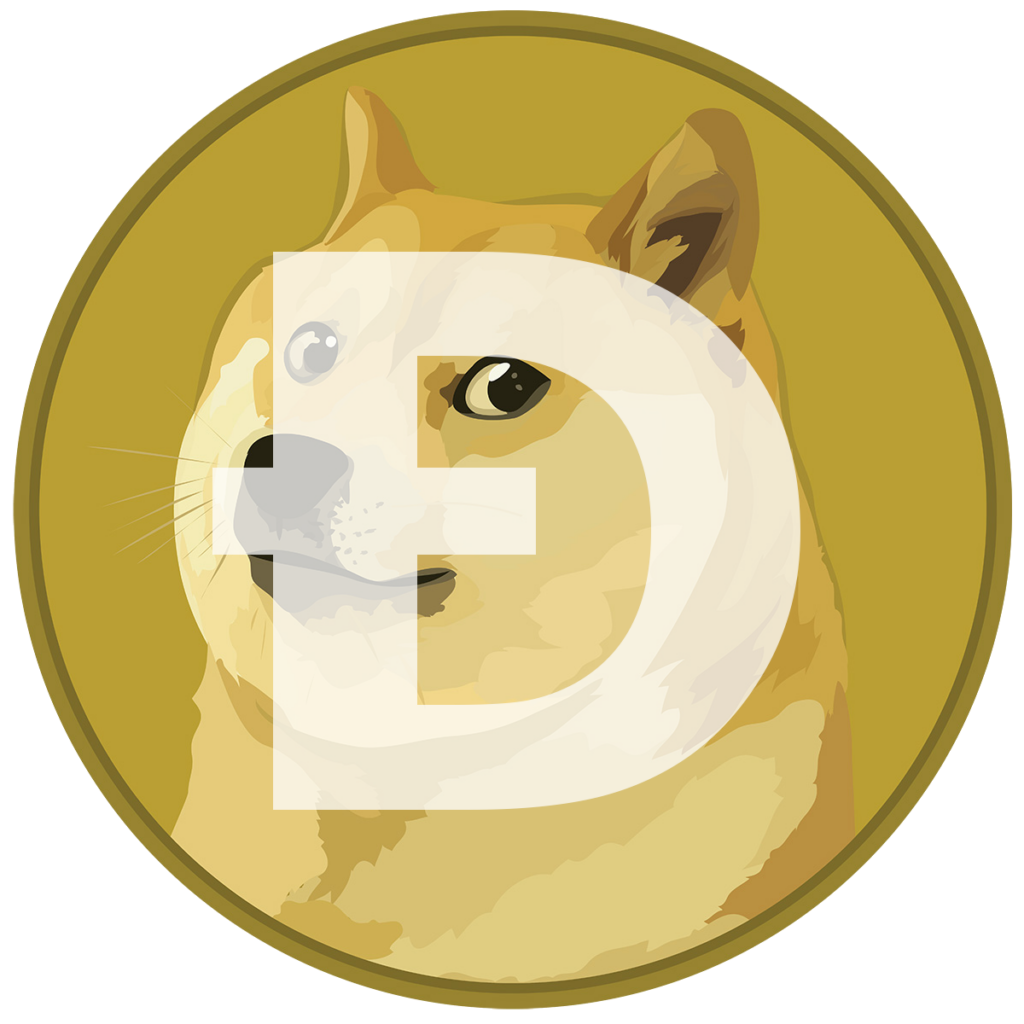
\includegraphics[width=1.5cm,height=1.5cm]{dogecoin.png}
		\caption{Dogecoin}
		\small URL : \url{https://block-builders.de/wp-content/uploads/2021/01/ony3qesa3ebx-1024x1024.png}
	\end{figure} 
	\begin{figure}[H]
		\centering
		
\includegraphics[width=1.5cm,height=1.5cm]{bitcoingold.png}
		\caption{Bitcoin Gold}
		\small URL : \url{https://s2.coinmarketcap.com/static/img/coins/200x200/2083.png}
	\end{figure} 

	Es gibt auch viele andere Kryptowährungen, die nicht auf Bitcoin basieren, aber die Proof-of-Work-Methode verwenden :
	
	\begin{figure}[H]
		\centering
		
\includegraphics[width=1.5cm,height=1.5cm]{ethereumclassic.png}
		\caption{Ethereum Classic}
		\small URL : \url{https://s2.coinmarketcap.com/static/img/coins/200x200/1321.png}
	\end{figure} 
	\begin{figure}[H]
		\centering
		
\includegraphics[width=1.5cm,height=1.5cm]{monero}
		\caption{Monero}
		\small URL : \url{https://s2.coinmarketcap.com/static/img/coins/200x200/328.png}
	\end{figure} 
	\begin{figure}[H]
		\centering
		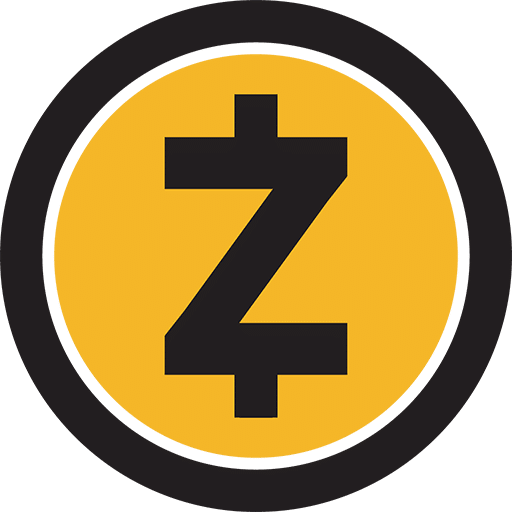
\includegraphics[width=1.5cm,height=1.5cm]{zcash}
		\caption{Zcash}
		\small URL : \url{https://z.cash/wp-content/uploads/2018/10/zcash-logo-fullcolor-512sq.png}
	\end{figure} 
	\begin{figure}[H]
		\centering
		
\includegraphics[width=1.5cm,height=1.5cm]{kadena}
		\caption{Kadena}
		\small URL : \url{https://s2.coinmarketcap.com/static/img/coins/200x200/5647.png}
	\end{figure} 

\section{Wie kann ich mit Kryptowährung Geld verdienen ?}
\subsection{Kryptowährungen und ihre produktive Seite: Eine Untersuchung des Krypto-Minings}
\subsubsection{Konzept}
Der aktuelle Marktwert von Bitcoin im Jahr 2022 liegt bei 15.891 Euro pro Einheit. Dies stellt einen hohen Preis für diese Kryptowährung dar und könnte für manche Personen oder Unternehmen von Interesse sein, die in das Mining von Bitcoin einsteigen möchten. Es ist jedoch wichtig zu beachten, dass das Bitcoin-Mining eine volatilen und riskanten Aktivität sein kann und gründliche Recherche und Planung erfordert, um erfolgreich zu sein.  \\ 
Ein Krypto-Mining-Rig ist ein spezielles Computersystem, das für das Mining von Kryptowährungen wie Bitcoin entwickelt wurde. Ein solches Rig besteht in der Regel aus einer Vielzahl von Computerkomponenten wie CPUs, GPUs, Motherboards, RAM und Speicher, die zusammengefügt werden, um eine möglichst hohe Rechenleistung zu erreichen. \\ 

Um ein erfolgreiches Krypto-Mining-Rig aufzubauen, ist es wichtig, eine geeignete Hardware auszuwählen, die leistungsfähig genug ist, um die erforderlichen Rechenaufgaben zu lösen, aber auch effizient genug, um die Energiekosten zu minimieren. Dazu gehört auch die Auswahl von Kühlsystemen, um die Hitzeentwicklung zu minimieren und die Lebensdauer der Hardware zu verlängern. \\
 
Ein Krypto-Mining-Rig ist ein spezieller Computer, der für das Mining von Kryptowährungen entwickelt wurde. Die Hardware, die für ein solches Rig benötigt wird, umfasst in der Regel eine leistungsstarke Hauptplatine, die mehrere Grafikkarten unterstützt, sowie eine robuste Stromversorgung, um die benötigte Rechenleistung zu gewährleisten. Es ist wichtig, dass das Rig über ausreichende Kapazitäten verfügt, um die hohen Anforderungen des Krypto-Minings erfüllen zu können, insbesondere bei hoher Konkurrenz und entsprechender Schwierigkeit. \\ 
Es ist von größter Bedeutung, dass man sich über die aktuellen Marktbedingungen und den Wert der Kryptowährungen informiert, in die investiert wird, um sicherzustellen, dass man das bestmögliche Preis-Leistungs-Verhältnis bei der Hardware-Auswahl erhält und das Rig weiterhin wirtschaftlich rentabel bleibt.
\cite{zdnet}
\newpage
\subsubsection{Hardware}
\begin{large}
	\textbf{Motherboard :} Asus B250 Mining Expert \\
	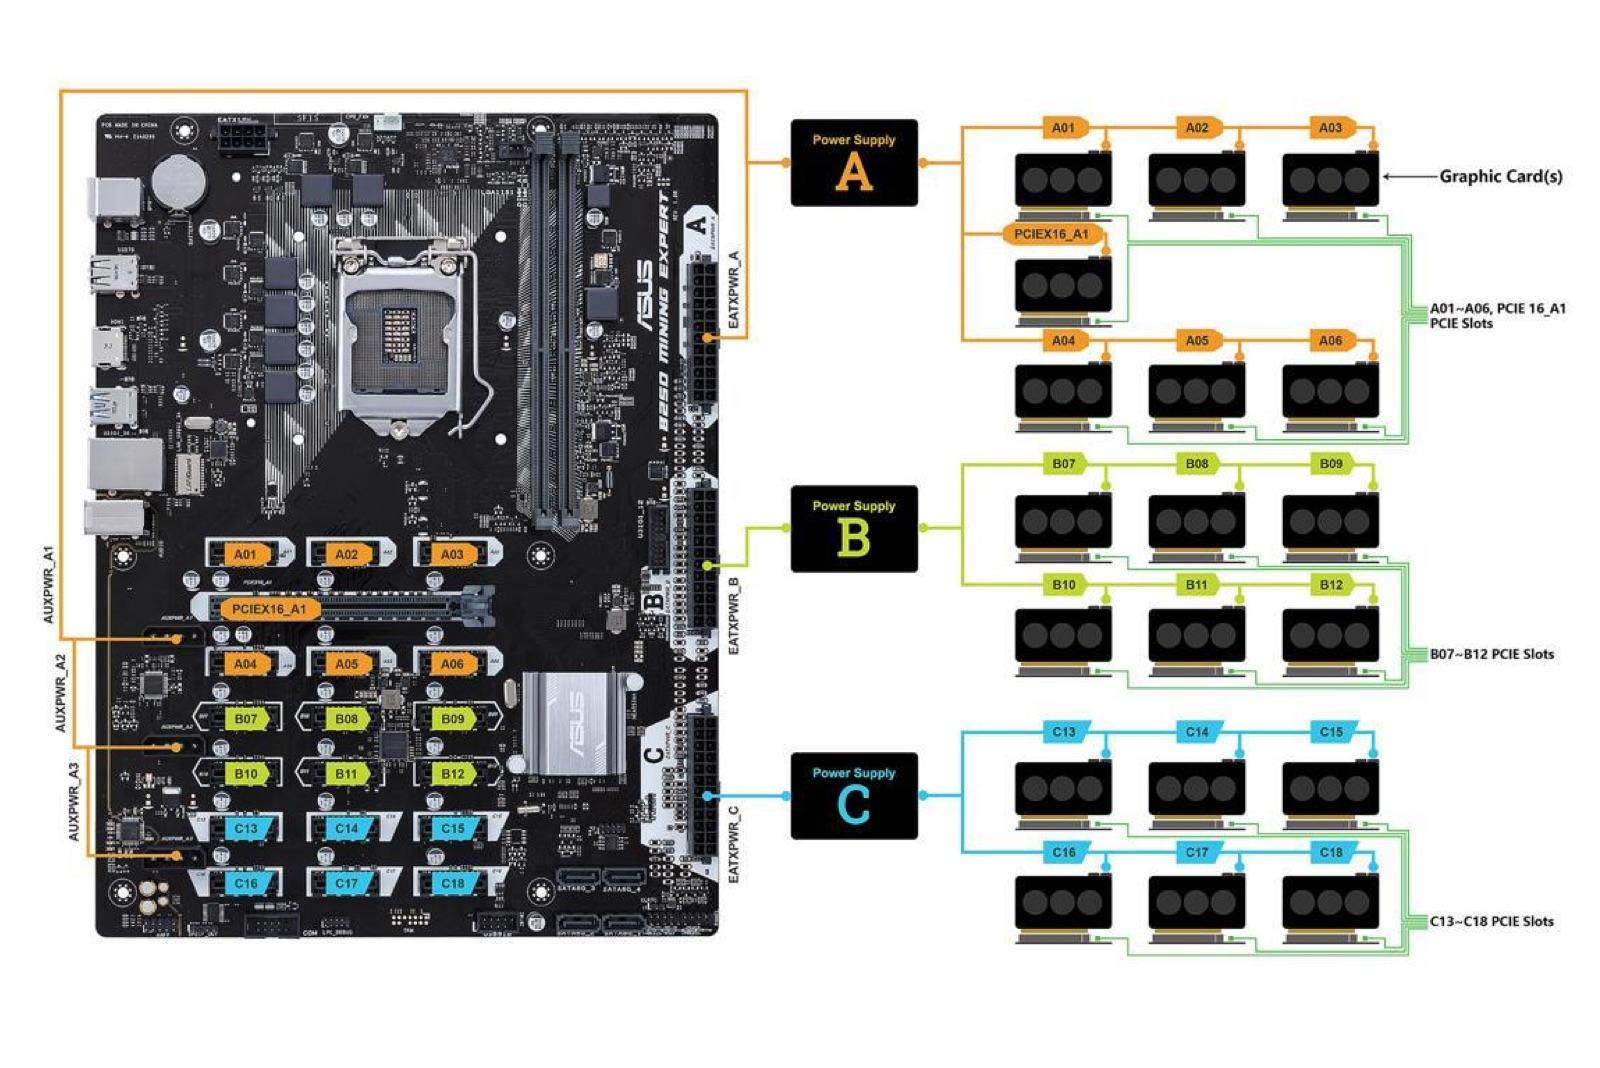
\includegraphics[width=15cm,height=15cm]{motherboard}  \\
	Das Motherboard, das in der Lage ist, 19 angeschlossene Grafikkarten zu verarbeiten, stellt eine leistungsstarke Hardware dar, die für das Krypto-Mining von Nutzen sein kann. Das Unternehmen Asus hat empfohlene GPU-Layouts für dieses Motherboard veröffentlicht, die für 19, 13 und 11 Grafikkarten vorsehen. Es kann jedoch auch mit anderen Layouts umgehen, obwohl es empfehlenswert ist, sich an den von Asus vorgeschlagenen Layouts zu orientieren, um optimale Leistung zu erzielen. \cite{zdnet}
	
\end{large}
\newpage
\begin{large}
	\textbf{CPU :} Intel Core i5-6500 \\ \\
	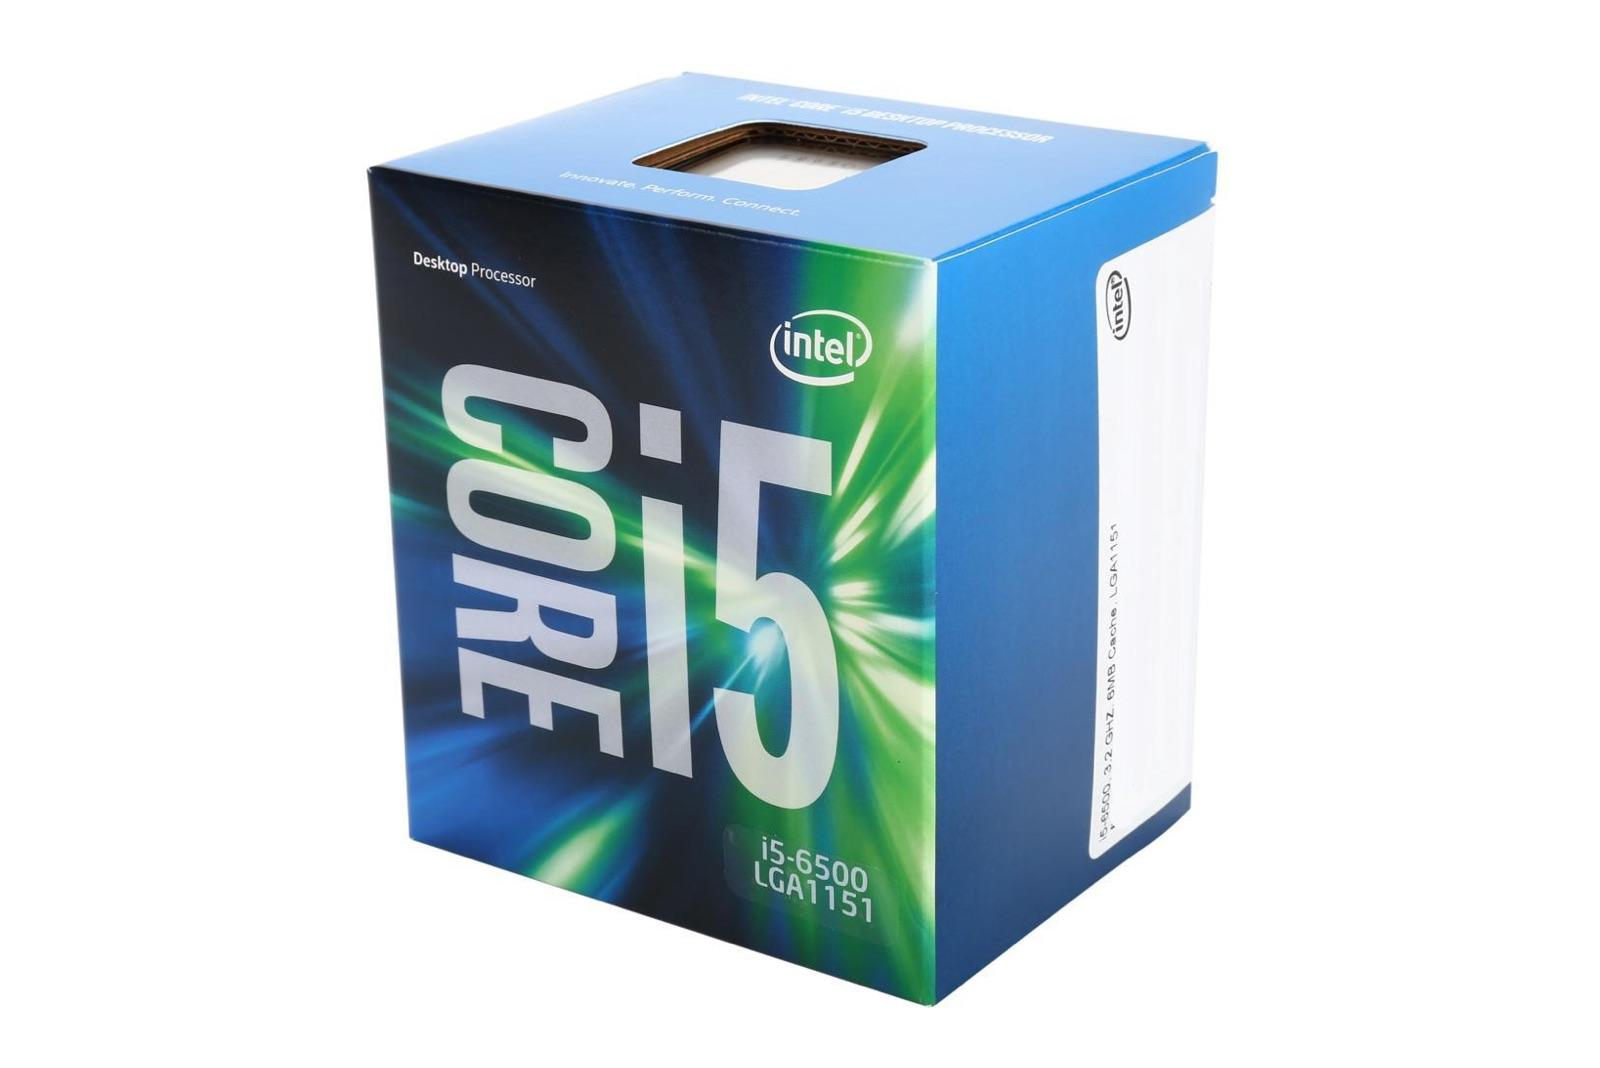
\includegraphics[width=10cm,height=8cm]{cpu}  \\ 
	Die Hauptprozessoreinheit, auch als CPU bezeichnet, wird auch für diese Einrichtung in Betracht gezogen, obwohl sie für das Mining an sich weniger von Bedeutung ist. Es ist jedoch wichtig, dass sie kompatibel mit dem Motherboard ist, um einen problemlosen Betrieb des Systems zu gewährleisten. \\ \\ \\
	
\end{large}
\begin{large}
	\textbf{RAM :} G.SKILL Aegis 16GB (2 x 8GB) \\ 
	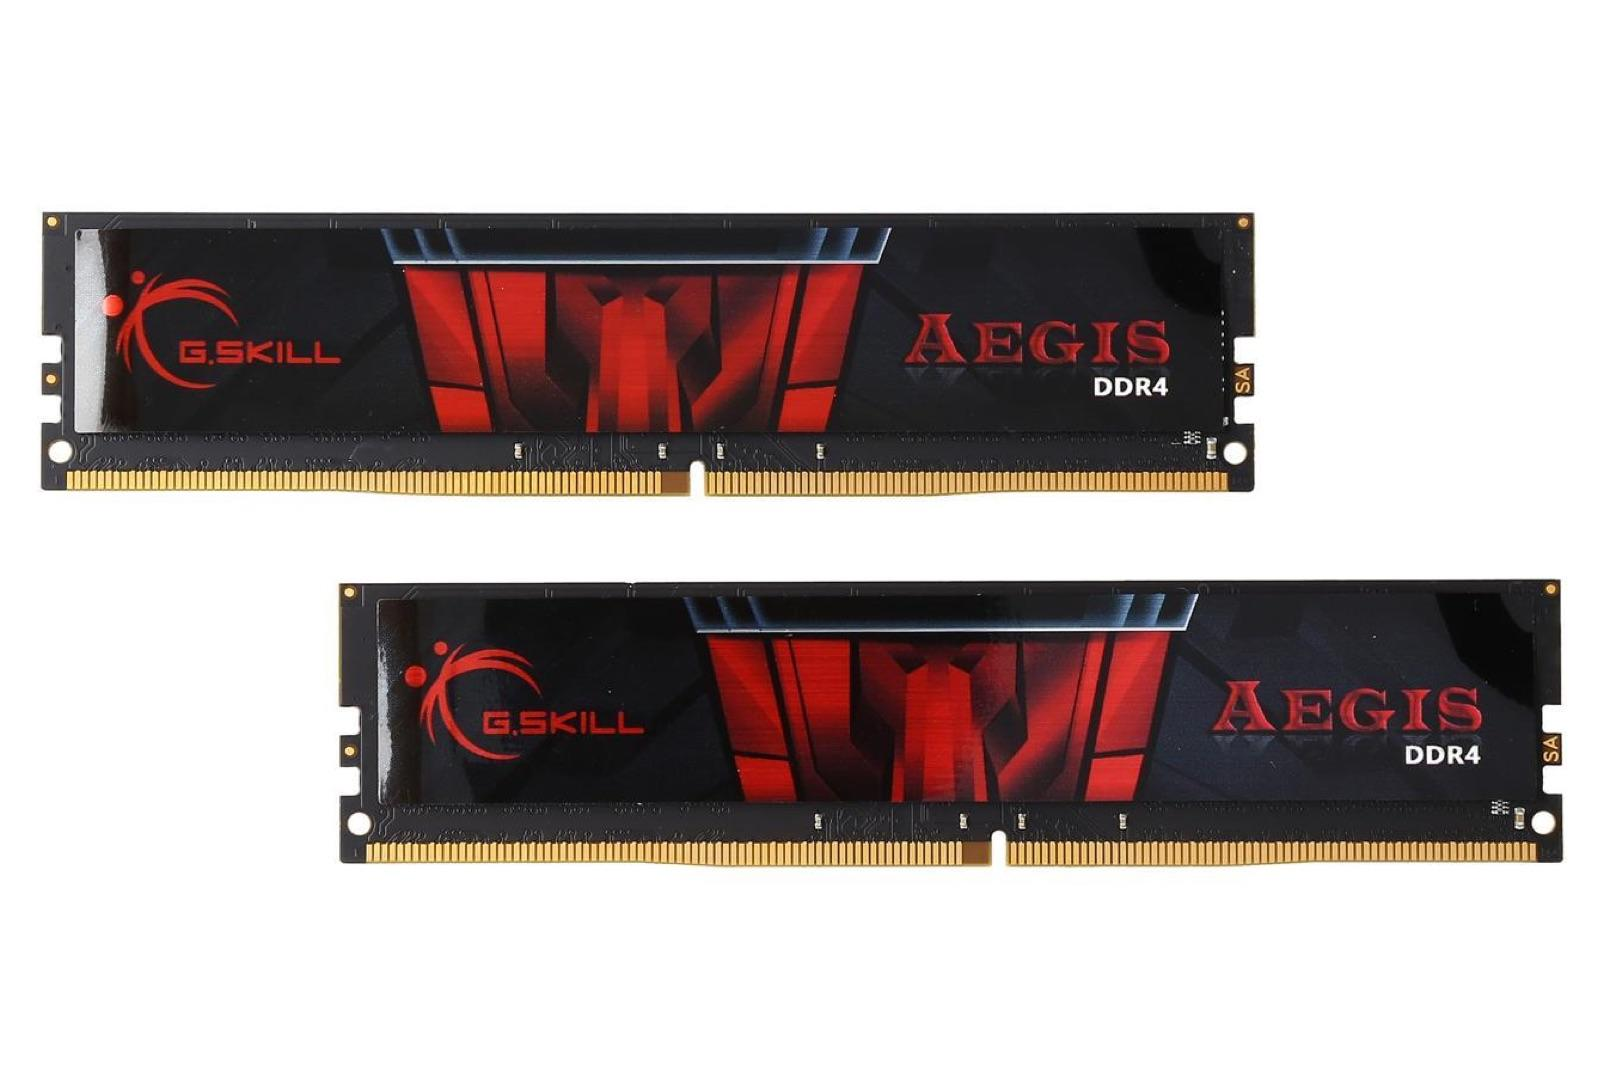
\includegraphics[width=\linewidth,height=5cm]{ram}  \\
	Für unsere Mining-Operationen ist es nicht notwendig, in einen enormen Vorrat an Arbeitsspeicher (RAM) zu investieren. Stattdessen reichen 16 GB DDR4-RAM aus, um unsere Ziele zu erreichen und den Betrieb unseres Unternehmens reibungslos zu gestalten. Es ist wichtig, sorgfältig abzuwägen, wie viel RAM benötigt wird, um unnötige Kosten zu vermeiden, ohne dabei die Leistungsfähigkeit des Systems zu beeinträchtigen. \\
	
\end{large}

\begin{large}
	\textbf{Storage :} SanDisk SSD Plus 1TB \\ 
	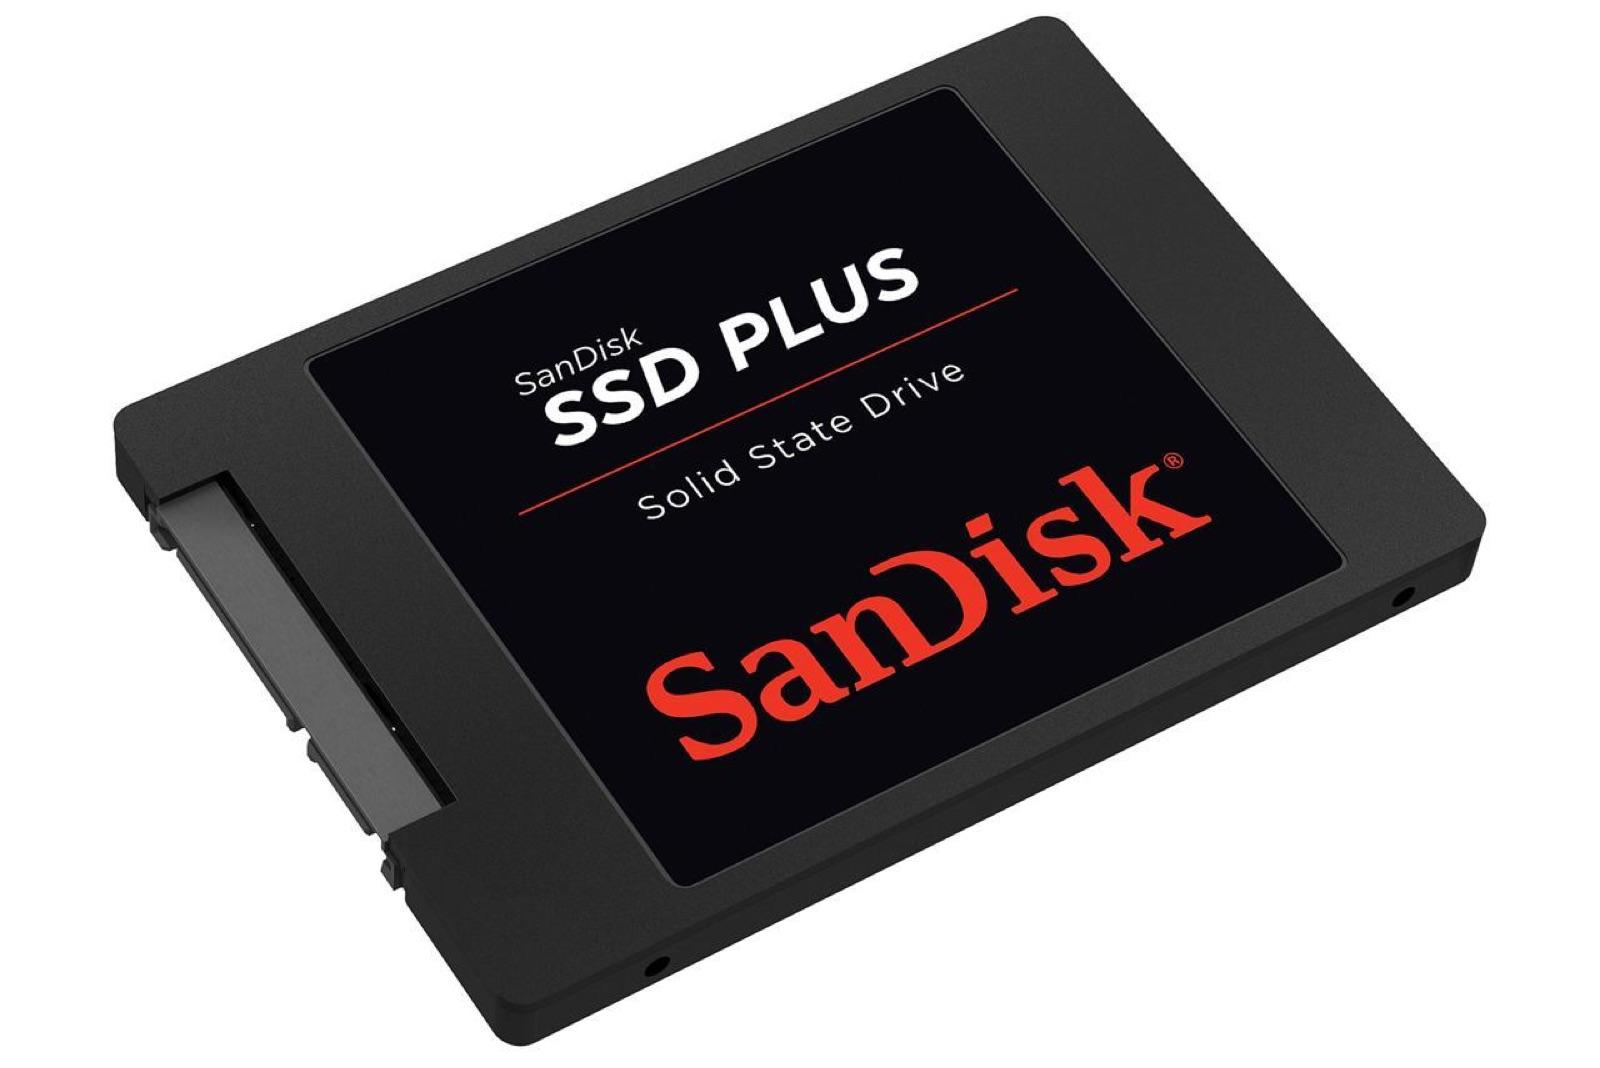
\includegraphics[width=\linewidth,height=5cm]{storage}  \\
	Die Verwendung von SSDs kann dazu beitragen, die Leistung des Mining-Rigs zu verbessern und den Betrieb zu beschleunigen. Es ist wichtig, sicherzustellen, dass die gewählten SSDs mit dem Motherboard kompatibel sind und genügend Speicherplatz für die Betriebsbedürfnisse des Unternehmens bereitstellen.	\\
\end{large}
\\ \\
\begin{large}
	\textbf{PSU :} Segotep 850W Full-Modular PSU \\ 
	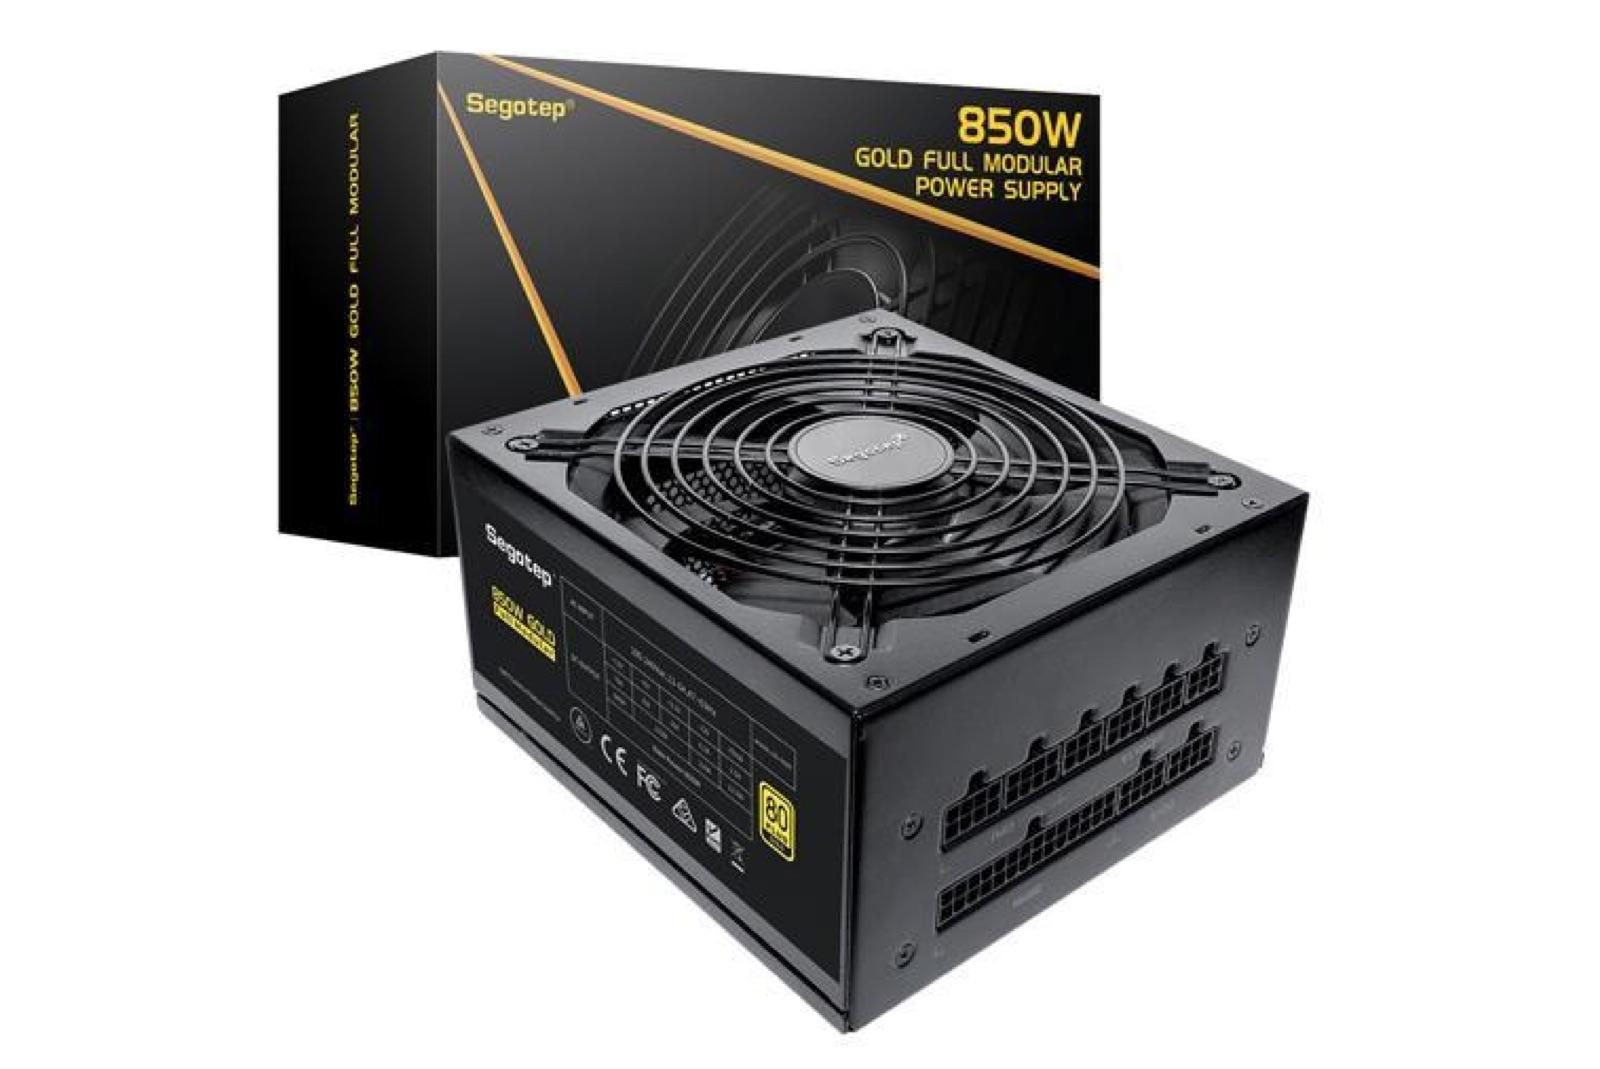
\includegraphics[width=\linewidth,height=5cm]{psu}  \\
	Es kann von Vorteil sein, mehrere "Segotep PSUs" zu verwenden, um sicherzustellen, dass ausreichend Leistung für das Krypto-Mining-Rig bereitgestellt wird, insbesondere wenn es mehrere Grafikkarten enthält. Allerdings ist es wichtig zu beachten, dass der Einsatz von mehreren PSUs auch mit höheren Kosten verbunden sein kann. Eine gründliche Überlegung der Leistungsanforderungen des Mining-Rigs und der dafür benötigten Stromversorgung kann helfen, die richtige Anzahl an PSUs und die damit verbundenen Kosten zu bestimmen. \\
\end{large}
\newpage
\begin{large}
	\textbf{PCI-e Riser :} FebSmart 16x to 1x Powered Riser 6-pack \\ 
	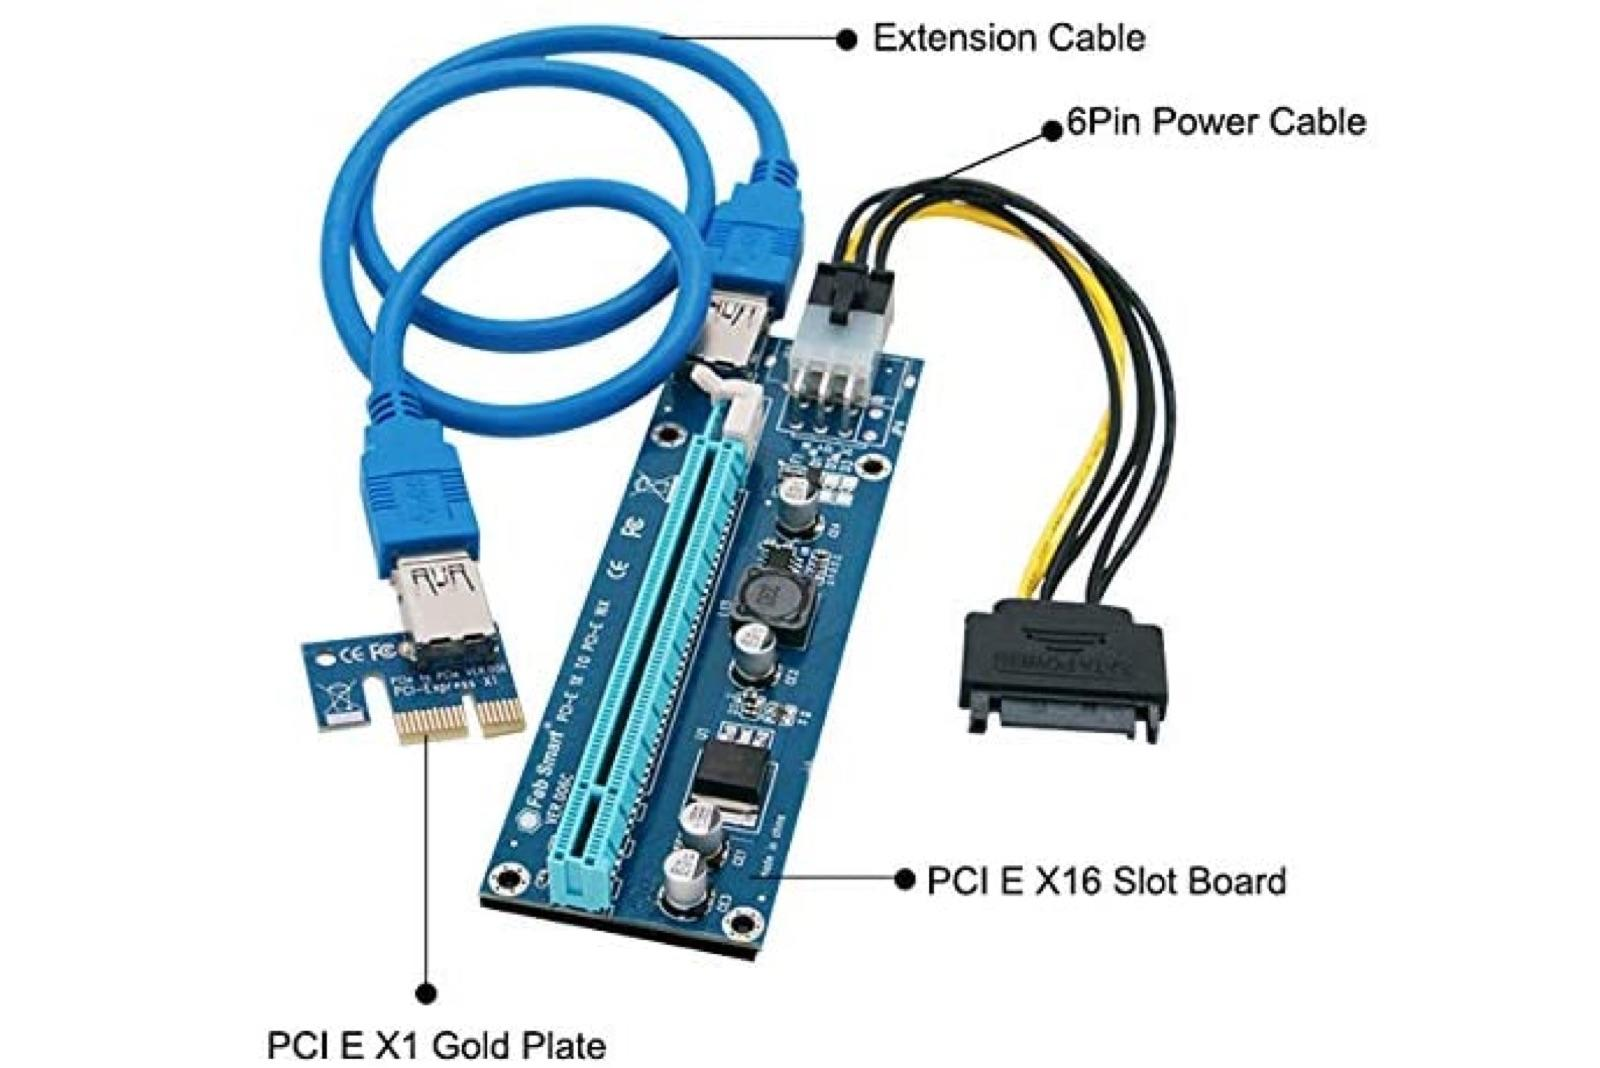
\includegraphics[width=\linewidth,height=5cm]{pci}  \\
	Das Verwenden von powered risers ist eine wichtige Überlegung bei der Einrichtung eines Krypto-Mining-Rigs, da sie es ermöglichen, die Grafikkarten indirekt an das Motherboard anzuschließen. Sie bieten auch eine stabile Stromversorgung für die Grafikkarten, um eine zuverlässige Leistung zu gewährleisten. Es ist wichtig zu beachten, dass der Bedarf an powered risers abhängig ist von der Anzahl der installierten Grafikkarten und dass es möglicherweise notwendig sein kann, mehrere von ihnen zu verwenden, um eine optimale Leistung zu erzielen. \\ \\ \\
	
	
\end{large}

\begin{large}
	\textbf{Nvidia graphics card :} MSI Ventus 3X GeForce RTX 3090
	 \\ 
	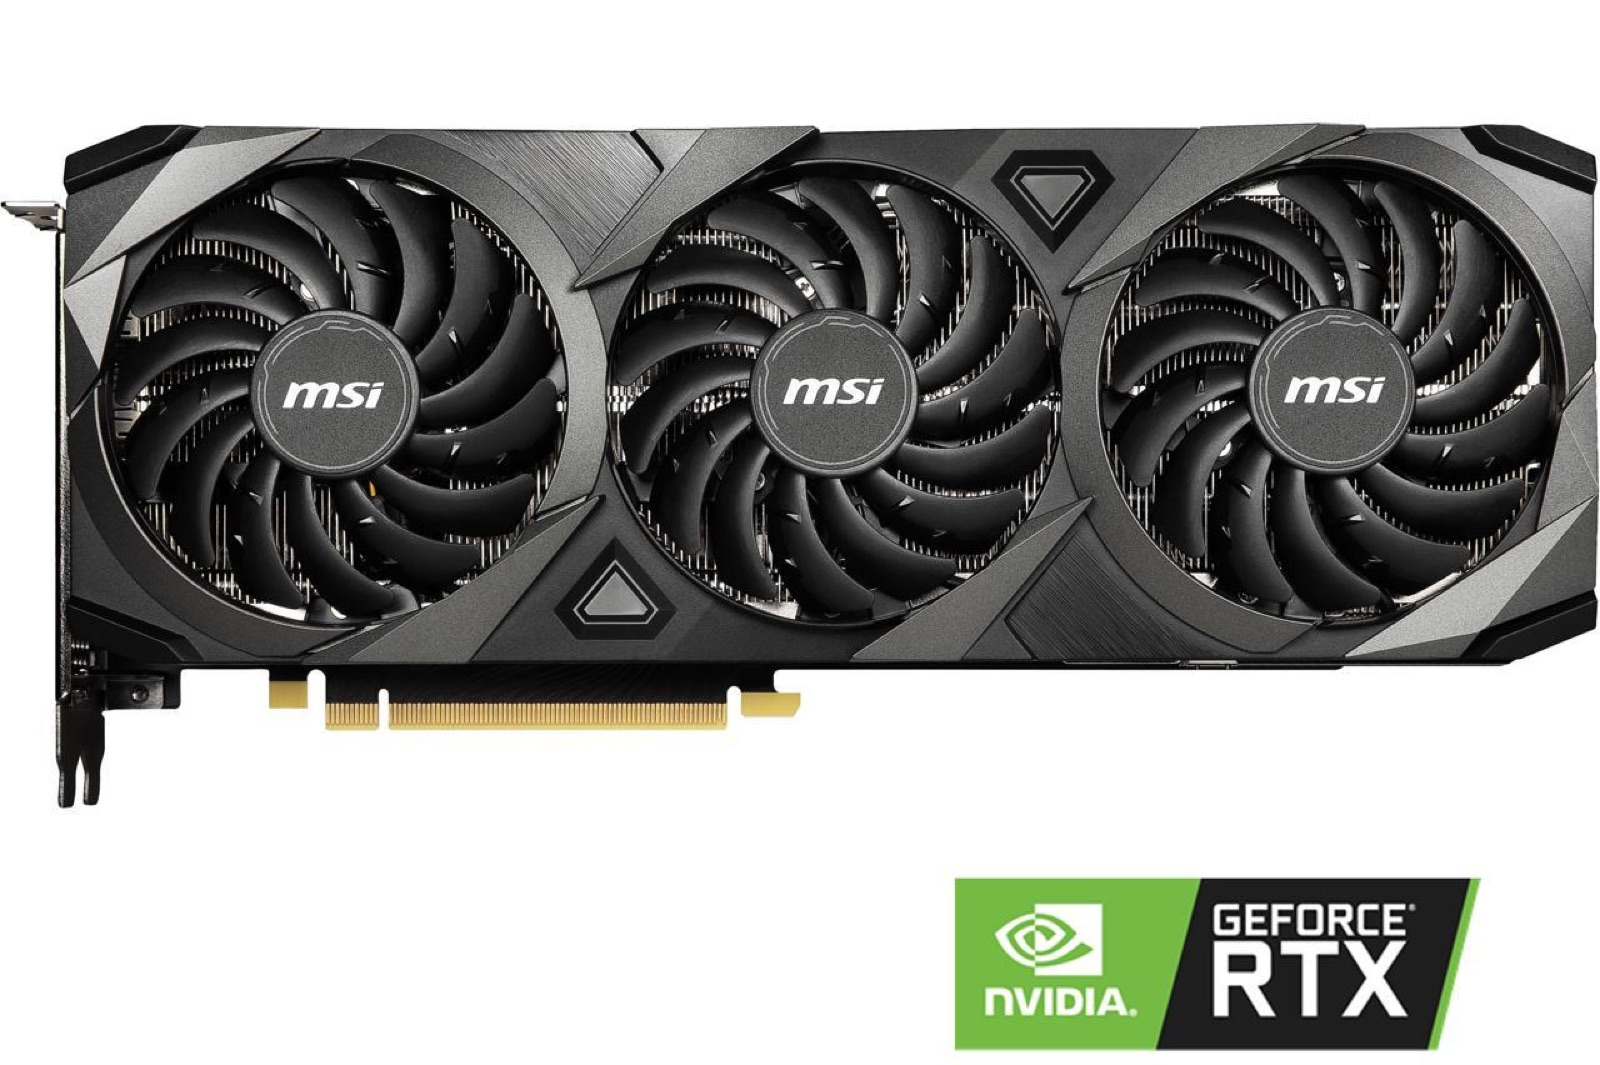
\includegraphics[width=\linewidth,height=5cm]{graphic}  \\
	Die Verwendung einer leistungsstarken Grafikkarte wie der beschriebenen ist für das Krypto-Mining von großer Bedeutung, da sie für die Verarbeitung von Rechenaufgaben und das Mining von Kryptowährungen verantwortlich ist. Diese spezifische Grafikkarte zeichnet sich durch ihre Fähigkeit zur Übertaktung, Stabilität und gute Kühlung aus. Sie ist auch bekannt für ihre Effizienz, was zu niedrigeren Stromkosten und reduzierten Bergbaukosten beitragen kann. Es ist wichtig, sich über die aktuellen Marktbedingungen und die Leistungsfähigkeit verschiedener Grafikkarten zu informieren, um die bestmögliche Wahl für das Krypto-Mining-Rig zu treffen. \\ 

\end{large}
\subsection{Wo sollte ich mein Geld in Kryptowährungen investieren?}
Es gibt einige Faktoren, die bei der Auswahl der nächsten erfolgreichen Kryptowährung berücksichtigt werden sollten. Dazu gehören die Skalierbarkeit der Blockchain, die Sicherheit der Technologie und die zugrunde liegende Idee, die von der Kryptowährung angegangen wird. Es ist auch wichtig, das Team hinter der Währung und ihre Erfolgsbilanz in der Vergangenheit zu betrachten. Es ist von großer Bedeutung, gründliche Recherchen durchzuführen und die damit verbundenen Risiken sorgfältig abzuwägen, bevor man in eine Kryptowährung investiert.
\cite{investopedia2} \cite{smartasset}
\begin{itemize}
	\item \textbf{Der Preis spielt eine wichtige Rolle bei der Entscheidung.}\\
	\textbf{Erklärung :} Eine wichtige Überlegung bei der Suche nach einer Kryptowährung ist der Preis des Tokens. Investoren, die nicht über ein großes Budget verfügen, können in Betracht ziehen, Kryptowährungen mit einem niedrigeren Preis zu erwerben. Es ist jedoch wichtig, dass Investoren gründliche Recherchen durchführen und Risiken sorgfältig abwägen, bevor sie in eine Kryptowährung investieren.
	
	
	\item \textbf{Es gibt gute Aussichten auf Annahme für die Kryptowährung, wenn sie von vielen Nutzern und Unternehmen akzeptiert wird.}\\
	\textbf{Erklärung :} Eine Kryptowährung, die einen wettbewerbsfähigen Vorteil gegenüber anderen bietet und von vielen Nutzern und Unternehmen akzeptiert wird, bietet gute Aussichten für eine erfolgreiche Investition. Es ist wichtig, sorgfältig die Eigenschaften und die Akzeptanz der Kryptowährung zu überprüfen, bevor man das eigene Geld investiert.
	
	
	\item \textbf{Die Versorgung ist ein Faktor, den man bei der Auswahl einer Kryptowährung berücksichtigen sollte.}\\
	\textbf{Erklärung :} Die Menge an Einheiten einer Kryptowährung, die momentan im Umlauf sind, wird als Versorgung bezeichnet. Eine geringere Versorgung könnte den Preis der Kryptowährung erhöhen, während eine höhere Versorgung möglicherweise dazu führt, dass der Preis sinkt. Bevor man in eine Kryptowährung investiert, ist es wichtig, sich über die Versorgung des Tokens zu informieren.
	
	
	
	\item \textbf{Preis und Volumen sind wichtig} \\
	\textbf{Erklärung :} In 2022 gibt es viele Plattformen, die das Investieren in Kryptowährungen vereinfachen, indem sie die wechselhafte Geschichte der Kryptowährungen und die Preise über den Blockchain-Markt verfolgen. Es ist daher ratsam, den Markt sorgfältig zu scannen und eine informierte Entscheidung über die Investition in Kryptowährungen zu treffen. Es gibt auch künstliche intelligente Modelle, die auf alten Kryptowährungsdaten basieren und es erleichtern, vorherzusagen, ob der Preis einer Kryptowährung in Zukunft steigen oder fallen wird. Allerdings sollte beachtet werden, dass der Preis von Kryptowährungen volatil ist und es immer das Risiko von Verlusten gibt. 
\end{itemize}


\chapter{Schluss}
Zusammenfassend lässt sich sagen, dass Bitcoin und andere Kryptowährungen durch den Einsatz des Konsensmechanismus "Proof-of-Work" validierte Transaktionen ermöglichen. Dieser Prozess erfordert starke Hardware-Ressourcen und kann durch das Mining von Belohnungen begleitet sein. Das Blockchain-Netzwerk spielt eine wichtige Rolle bei der Überprüfung der Gültigkeit von Transaktionen und der Aufrechterhaltung der Integrität des Systems. Vor dem Investieren in Bitcoin oder eine andere Kryptowährung ist es wichtig, sich über den Markt und die verschiedenen Optionen gründlich zu informieren und das Risiko sorgfältig abzuwägen.\\ \\

Die Perspektiven für Proof-Of-Work und andere Konsensmechanismen in der Kryptowährungswelt sind derzeit ungewiss. Proof-Of-Work ist derzeit der am weitesten verbreitete Konsensmechanismus und wird von vielen Kryptowährungen wie Bitcoin und Ethereum verwendet, aber es hat auch einige Nachteile, wie hohe Energiekosten und langsame Transaktionsgeschwindigkeiten, die zu einer eingeschränkten Skalierbarkeit führen. \\

Es gibt auch andere Konsensmechanismen, wie Proof-Of-Stake, die derzeit entwickelt werden und möglicherweise eine Alternative zu Proof-Of-Work darstellen könnten. Proof-Of-Stake erfordert von Teilnehmern, eine bestimmte Menge an Kryptowährung zu "staken", um als Miner zu fungieren, was zu reduzierten Energiekosten führen könnte. Es gibt jedoch noch Fragen hinsichtlich der Sicherheit von Proof-Of-Stake und ob es die gleiche Sicherheit wie Proof-Of-Work gewährleisten kann.\\ 

Es ist unmöglich vorherzusagen, welcher Konsensmechanismus in Zukunft dominieren wird. Es ist jedoch wichtig, dass Kryptowährungen kontinuierlich verbessert werden, um Skalierbarkeit und Sicherheit zu verbessern. Es ist auch wahrscheinlich, dass es in der Zukunft weitere neue Konsensmechanismen geben wird, die die Landschaft der Kryptowährung verändern könnten. Eines dieser Konsensmechanismen, das zunehmend in den Fokus gerät, ist Proof-Of-Authority. Dieser Mechanismus basiert auf einem Netzwerk von autorisierten Validatoren, die Transaktionen bestätigen und das Netzwerk sicher halten. Proof-Of-Authority könnte eine günstigere und schnellere Alternative zu Proof-Of-Work darstellen, aber es gibt auch Bedenken bezüglich der Zentralisierung und der möglichen Einflussnahme von Validatoren. Es ist wichtig, dass die Entwickler weiter an neuen und verbesserten Mechanismen arbeiten, um die Effizienz und Sicherheit von Kryptowährungen zu gewährleisten. Investoren sollten sich über die verschiedenen Konsensmechanismen informieren und Risiken sorgfältig abwägen, bevor sie in Kryptowährungen investieren.

\printbibliography


\end{document}
